\documentclass[10pt]{reportMaster}
\usepackage[a4paper]{geometry}
\usepackage{graphicx}
\usepackage{amsmath}
\usepackage{algorithm}
\usepackage{algpseudocode} 
\usepackage[titletoc]{appendix}
\DeclareMathOperator*{\argmax}{arg\,max}
\DeclareMathOperator*{\argmin}{arg\,min}
\setlength{\footskip}{100pt}
\usepackage{amsfonts}
\usepackage{multirow}
\usepackage[hidelinks]{hyperref}

%%% The title of the thesis, and the author (astudent) of the thesis
\title{Optimization of Transductive Conformal Predictors based on Naive Bayes Classifier via Incremental and Decremental Learning}
\author{Zhize Guan}

%%% Uncomment the line with the Master program of the student
% \nameMastersProgramme{Artificial Intelligence}
\nameMastersProgramme{Data Science for Decision Making}  

%%% Here, write the department supervisor(s), as well as all department examiners; 
%%% Write also any external supervisor(s), if applicable
\committee{Dr. Evgueni Smirnov \\ Dr. Rachel Cavill}
\date{\today}

\begin{document}
\maketitle

\begin{abstract}
Transductive Conformal Predictors (TCP) offer prediction sets in Machine Learning (ML) problems, making them more desirable than conventional point predictors. However, their extensive computational complexity during the Leave-One-Out (LOO) procedure significantly restricts their applicability to large datasets. To overcome this limitation, we propose the utilization of Incremental and Decremental Learning (I\&D Learning). Specifically, we propose a specific TCP that employs the Naive Bayes Classifier (NBC) as the underlying ML method and enhance its performance. To accommodate different types of data variables, we design two variations of NBC for optimization: MultinomialNB for discrete variables and GaussianNB for continuous variables. Experimental results demonstrate a drastic reduction in prediction time, by at least one order of magnitude, while maintaining identical solutions to the non-optimized methods. Additionally, we conduct exploratory experiments to compare the computational performance of our optimized methods with other TCP that employ the same improvement strategy.

\end{abstract}

\newpage
\tableofcontents

\cleardoublepage
\addcontentsline{toc}{chapter}{\listfigurename}
\listoffigures
\cleardoublepage
\addcontentsline{toc}{chapter}{\listtablename}
\listoftables
\cleardoublepage
\addcontentsline{toc}{chapter}{\listabbrname}
\listofabbrs

\noindent \textbf{ML}  Machine Learning \\\\
\noindent \textbf{NBC}  Naive Bayes Classifier \\\\
\noindent \textbf{MultinomialNB} Multinomial Naive Bayes Classifier\\\\
\noindent \textbf{GaussianNB}  Gaussian Naive Bayes Classifier\\\\
\noindent \textbf{LOO} Leav-One-Out \\\\
\noindent \textbf{NM}  Nonconformity Measure \\\\
\noindent \textbf{NMS}  Nonconformity Measure Score \\\\
\noindent \textbf{CP}  Conformal Predictor \\\\
\noindent \textbf{ICP}  Inductive Conformal Predictor \\\\
\noindent \textbf{TCP}  Transductive Conformal Predictor \\\\
\noindent \textbf{I\&D Learning}  Incremental and Decremental Learning \\\\
\noindent \textbf{i.i.d.} Independently and Identically Distributed \\\\
\noindent \textbf{TCP:C} Transductive Conformal Predictor based on Classifier C\\\\
\noindent \textbf{OTCP:C} Optimized Transductive Conformal Predictor based on Classifier C\\\\




\chapter{Introduction}

\section{Motivation}
In Machine Learning (ML), the common form of classification methods focuses on point estimation, aiming to provide the best possible class label for a test instance \cite{johansson2013evolved, vanderlooy2006analysis}. However, in real-world applications where the cost of misclassification is extremely high, it becomes necessary to estimate a prediction set that contains potential classes for a given test instance $x$, instead of a single-point estimate. Various types of set predictors have been proposed, all aiming to possess two essential properties: validity and informational efficiency. Validity means that the probability of the prediction set not containing the class for the test instance $x$ is no greater than the chosen significance level $\epsilon$. Efficiency, on the other hand, refers to the set being both non-empty and small in size.\\

\noindent The conformal prediction, proposed by Vovk \cite{vovk2005algorithmic} enables the prediction set to satisfy the validity criterion automatically. In this framework, the decision of whether to include class $y$ in the set for a test instance $x$ is based on computing nonconformity measure scores. The process involves calculating the p-value $p(x,y)$ for class $y$, which represents the proportion of instances with nonconformity scores greater than or equal to that of the instance $(x, y)$. If the $p(x,y)$ exceeds the chosen significance level $\epsilon$, the class $y$ is added to the prediction set. A nonconformity measure score assigned to a labelled instance reflects how untypical is the instance compared to the remaining instances in the dataset. Typically, nonconformity measure functions are designed for specific point predictors. In addition to validity, another significant advantage is that conformal prediction does not require strict assumptions on the data distribution, and we only need to assume that the training instances are exchangeable, a weaker requirement than the Independently and Identically Distributed (i.i.d.) assumption. \\

\noindent Transductive Conformal Predictors (TCP) are the most original Conformal Predictors (CP). Apart from the advantages mentioned above, they are known to have better predictive efficiency than other CP, but the high computational complexity of computing nonconformity score for all instances restricts its practicality when dealing with large datasets. In the context of classification, let's consider a scenario where the size of the training dataset $D$ is denoted as $N$. The class variable $Y$ represents discrete values, and there are $|Y|$ possible class labels $y$. In this case, we select a possible class label $y$ and combine it with the test instance $x$ to create the labelled instance $(x, y)$. Subsequently, we combine $(x,y)$ with the training dataset $D$ to get a new dataset of $(N+1)$ instances and then iterate through each instance of the new dataset, using one instance at a time as the test instance, while the remaining $N$ instances serve as the training dataset $\Tilde{D}$ for the ML method. During the training step, the ML method is trained on $\Tilde{D}$, and subsequently, the trained model is employed to predict the test instance. The score is then computed based on the predicted value. Therefore, the Leave-One-Out (LOO) procedure requires the ML method to be trained $(N+1)$ times in order to calculate scores for $(N+1)$ instances. Considering that there are $|Y|$ possible classes, we need to multiply by $|Y|$ and get the final result $(N + 1) \cdot |Y|$.\\

\noindent In order to reduce the running time, a new method has been processed to speed up a TCP by studying it in conjunction with the underlying ML method and by exploiting Incremental and Decremental Learning (I\&D Learning). 

\section{Related Work}
TCP have great predictive efficiency, but they become unfeasible for most applications due to their high computational complexity during the LOO procedure. As a result, researchers have been exploring alternatives in order to decrease computational complexity. \\

\noindent One approach is decreasing the training dataset to reduce complexity, which is called Sampling Learning. For example, the modified version of TCP called Inductive Conformal Predictors (ICP) \cite{vovk2005algorithmic, papadopoulos2002inductive} train the ML method on a subset of the training dataset. This modification avoids the computationally expensive LOO step but does affect the predictive power. Other approaches have been proposed to address the statistical inefficiency of ICP while maintaining favourable computational complexity. One such idea is cross-CP \cite{vovk2015cross}, which takes into account the cross-correlations between the output variable and the input variables during the prediction process. By considering these cross-correlations, cross-CP aims to enhance the accuracy and reliability of predictions in conformal prediction. Another technique, known as CV+ \cite{barber2021predictive}, combines the principles of cross-validation and conformal prediction. By utilizing cross-validation, CV+ divides the dataset into subsets, using each subset as a validation set while the remaining data is used for training. Similarly, jack-knife+ \cite{barber2021predictive} integrates the jackknife resampling technique with conformal prediction. By iteratively leaving out one instance from the training set and retraining the model on the remaining instances, jack-knife+ takes advantage of resampling to improve the robustness and reliability of predictions. These approaches aim to address the statistical inefficiency of ICP by incorporating additional considerations, such as cross-correlations and resampling techniques, while still maintaining computational efficiency. However, they do result in lower prediction efficiency compared to TCP. Thus, having access to efficient optimizations of TCP becomes crucial for applications that demand high statistical efficiency and performance \cite{lei2019fast}.\\

\noindent TCP can be constructed for any ML method, so we can transform the method into a scoring function, known as the nonconformity measure. In simple terms, this function quantifies the degree of dissimilarity of a test instance with respect to the training instances. Based on the ML methods which can be both incremental and decremental, another optimization approach called Online Learning is proposed. The authors \cite{cherubin2021exact} observe that, in order to speed TCP up, the nonconformity measure should be able to efficiently both learn a new instance and unlearn an old instance. Thus, they use this idea to produce the exact optimization of TCP for  k-Nearest Neighbors (k-NN), Kernel Density Estimation (KDE), and kernel Least-Squares SVM (LS-SVM). All these reduce the complexity by at least one order of magnitude. Further, they demonstrate that similar ideas can lead to marginal improvements in bootstrapping methods and expand the techniques to CP regression. 

\section{Research Questions}

Taking inspiration from Online Learning, we aim to develop an optimized variant of TCP that utilizes the Naive Bayes classifier (NBC) as its underlying ML method. The main idea is to efficiently compute the Nonconformity Measure Score (NMS) when learning a new instance and unlearning an old instance. Specifically, within the framework of Naive Bayes, our objective is to update the estimates of the probabilities $P(y)$ and $P(x|y)$ quickly.\\

\noindent In this thesis, we propose two optimized TCP utilizing NBC, designed specifically for discrete and continuous variables, respectively. We will examine their consistency with standard TCP and compare their computational performance in terms of running time. Additionally, we will conduct a thorough time complexity analysis to compare our proposed methods with standard and other optimized TCP. Through experiments, we aim to determine the fastest approach. Addressing these concerns, our research focuses on three primary research questions:

\begin{itemize}
\item Can the optimized Transductive Conformal Predictors based on Naive Bayes Classifier produce the same exact solutions as standard ones?
\item Can the optimized Transductive Conformal Predictors based on Naive Bayes Classifier reduce the training time and prediction time significantly?
\item Can the optimized Transductive Conformal Predictors based on Naive Bayes Classifier reduce more training time and prediction time than other optimized TCP based on different ML methods?
\end{itemize}

\section{Scope and Limitation}
Due to the fixed time frame, some limitations have to be set on this research to ensure the
work can be finished in time.

\begin{itemize}

\item This work primarily focuses on the optimization of TCP based on NBC as the underlying ML method for classification problems. Additionally, we include a direct comparison with other optimized TCP that employ the k-NN and KDE algorithms, as presented in a referenced paper \cite{cherubin2021exact}.

\item In this study, we focus solely on implementing NBC for datasets with either complete discrete or continuous variables. We do not consider the case of mixed variables. Additionally, we acknowledge that our implementation does not account for instances where certain variables are absent in the training dataset, resulting in zero probabilities during computations for discrete variables.

\end{itemize}

\section{Outline}

The upcoming Chapter 2 will provide a thorough theoretical background, focusing on the introduction to the Classification Problem, Naive Bayes Classifier, and Conformal Prediction. Moreover, it will also encompass a discussion on the standard TCP utilizing NBC. In Chapter 3, we will present our primary contributions, which revolve around the optimized TCP utilizing NBC. This chapter will delve into the detailed methodology and include a comprehensive analysis of the time complexity for all TCP mentioned. Subsequently, Chapter 4 will showcase the datasets used, the experimental setup, and the results obtained. A detailed discussion and analysis of these experiments will be provided. Readers interested in the code implementation can find it at the link below\footnote[1]{The python code implementation can be found at \url{https://github.com/zhizeguan/Optimization-of-TCP-based-on-NBC-via-Incremental-and-Decremental-Learning}}. Finally, Chapter 5 will summarize the work conducted in this study and offer insights into potential future research directions and expansions related to this topic.

\chapter{Methods}

This chapter begins by introducing the Classification Problem. Then, it provides a comprehensive overview of the Naive Bayes Classifier, followed by two specific types. The final section introduces the concept of Conformal Prediction and TCP based on NBC are demonstrated.

\section{Classification Problem}

In this section, we analyse classification problems from a Bayes View. Let $X$ be an instance space defined by $P$ input variables $X^p$, $Y$ be a finite discrete output variable, and $Q$ be some unknown joint probability distribution over $X \times Y$. The training dataset $D$ of size $N$ is sampled from $X \times Y$ under the i.i.d. assumption. We want to find the most probable class label $y \in Y$ for a test instance $x \in X$ according to $Q$.\footnote[2]{In our notation: $X^p$ is the $p$-th input variable, $x_n^p$ is the value for $n$-th instance’s $p$-th input variable, and $y_n$ is the class for $n$-th instance.}\\

\noindent Each tuple $(x,y)$ in $X \times Y$ is a value of a random variable $Z$ defined over $X \times Y$ by the probability distribution $Q$. If we sample with replacement from $X \times Y$ according to the probability distribution $Q$, we receive the training dataset $D$, which equals to $\{(x_1, y_1),(x_2,y_2),...,(x_N,y_N)\}$. Thus, $D$ is a realization of $N$ random variables $Z_n$. We assume that (1) the random variables $Z_n$ are independent, and (2) the random variables $Z_n$ are identically distributed. Independent sampling ensures that training instances are selected independently according to the unknown distribution $Q$, so we do not need to model the dependency between training instances in the training dataset $D$. Identically distributed sampling ensures that the test instance to be classified will be generated by the same distribution $Q$. Thus, we have a bridge between the past (the training dataset $D$) and the future (the test instance to be classified).\\

\noindent To solve the classification problem for a test instance $x \in X$, we can assume that we know:
\begin{itemize}
\item the prior distribution $P(y)$
\item the distribution $P(x|y)$ for each $y \in Y$
\item the distribution $P(x)$
\end{itemize}
Then, we can compute the posterior probability $P(y|x)$ for each $y \in Y$ according to the Bayes Rule:
\begin{equation}
    P(y|x) = \frac{P(x|y)P(y)}{P(x)} \tag{1}\label{eq:1}
\end{equation}

\noindent The winning class is determined by the Optimal Bayes Rule:

\begin{equation}
    \hat{y} &= \argmax_{y \in Y} P(y|x)\tag{2}\label{eq:2}
\end{equation}

\section{Naive Bayes Classifier}
\subsection{Introduction}
Naive Bayes Classifiers (NBC) are a series of supervised machine learning classification algorithms that utilize Bayes' theorem with the "naive" assumption of independence between each pair of variables. NBC do not employ any search in a hypothesis space; they just multiply probability estimates.

\begin{subequations}
\begin{align}
    \hat{y} &= \argmax_{y \in Y} P(y|x) \tag{3a}\label{eq:3a}\\
            &= \argmax_{y \in Y} \frac{P(y)P(x|y)}{P(x)}\tag{3b}\label{eq:3b}\\
            &= \argmax_{y \in Y} \frac{P(y)P(x_1,...,x_P|y)}{P(x_1,...,x_P)}\tag{3c}\label{eq:3c}\\
            &= \argmax_{y \in Y} \frac{P(y)\prod_{p=1}^{P} P(x_p|y)}{P(x_1,...,x_P)}\tag{3d}\label{eq:3d}\\
            &= \argmax_{y \in Y} P(y) \prod_{p=1}^{P} P(x_p|y)\tag{3e}\label{eq:3e}
\end{align}
\label{eq:2} 
\end{subequations}\\

\noindent According to Equation (1) in the last section, we can convert the step (\ref{eq:3a}) to get step (\ref{eq:3b}). Next, we use the naive conditional independence assumption, which assumes that the input variables are conditionally independent: $P(x_p|y,x_1,...,x_{p-1},x_{p+1},...,x_P)=P(x_p|y)$ to simplify the step (3c) and get the next step (\ref{eq:3d}). Besides, since $P(x_1,...,x_P)$ is constant given the test instance, we can simplify the equation a little bit more and get the final step (\ref{eq:3e}). $P(y)$ is the relative frequency of class $y$ in the training dataset. NBC differ mainly by the assumptions they make regarding the distribution of $P(x_p|y)$.\\

\noindent NBC are defined by step (\ref{eq:3e}). They estimate the probabilities $P(y)$ and $P(x_p|y)$ from the training dataset. Despite the unrealistic naive assumption made, they show remarkable success in practice and are used to compete with much more advanced methods \cite{hilden1984statistical, langley1992analysis}. Besides, NBC have proven effective in many practical applications, including text classification, medical diagnosis, and systems performance management \cite{domingos1997optimality, hellerstein2000recognizing, mitchell1997artificial}. Two specific NBC for discrete and continuous variables are provided in Subsections \ref{section:2.2.2} and \ref{section:2.2.3}.

\subsection{MultinomialNB for Discrete Variables} \label{section:2.2.2}

In order to implement the NBC for discrete variables, Multinomial Naive Bayes Classifier (MultinomialNB) is presented in Algorithm \ref{alg:MultinomialNB}. The algorithm input consists of a training dataset $D$, which contains $N$ instances with $P$ input variables $X^p$ and output variable $Y$, and a test instance $x_{N+1}$.\\ 

\noindent Firstly, the initialization step involves setting the values of two types of counters, namely $C[y]$ and $C[y, X^p,x]$, to zero. Subsequently, during the training step, counter $C[y]$ is responsible for storing the count for class $y$, while $C[y, X^p,x]$ maintains the count for class $y$, variable $X^p$, and value $x$. Moving on to the prediction step, the algorithm computes the estimated prior $\hat{P}(y)$ by dividing $C[y]$ by the total number of instances $N$. Similarly, the likelihood $\hat{P}(x_{N+1}^p|y)$ is calculated by dividing $C[y, X^p, x_{N+1}^p]$ by $C[y]$. These estimated probabilities are then multiplied together to obtain the posterior $\hat{P}(x_{N+1},y)$ for each class $y$. Finally, the predicted class $\hat{y}$ with the highest posterior probability for the test instance is determined as the class. It is important to note that the training step of MultinomialNB only requires execution once, whereas the prediction step needs to be repeated multiple times for different test instances.

\begin{algorithm}[H]
\caption{MultinomialNB}\label{alg:MultinomialNB}
\textbf{Input:} \; \; Training dataset $D$ of $N$ instances, $P$ input variables $X^p$ and output variable $Y$.\\
\hspace*{\algorithmicindent} \quad \quad \; \; Test instance $x_{N+1}$.\\
\textbf{Output:} \,  Estimated posterior probability distribution $\{ \hat{P}(x_{N+1},y)\}_{y \in Y}$.\\
\hspace*{\algorithmicindent} \quad \quad \; \; Estimated class $\hat{y}$ for test instance $x_{N+1}$.

\begin{algorithmic}[1]
\State // Initialization
\State \textbf{for each class} $y \in Y$ \textbf{do}
\State \qquad $C[y] := 0$
\State \qquad \textbf{for each input variable} $X^p$ \textbf{do}
\State \qquad \qquad \textbf{for each value} $x$ of $X^p$ \textbf{do}
\State \qquad \qquad \qquad $C[y,X^p,x] := 0$
\State // Training
\State \textbf{for each} $(x_n,y_n) \in D$ \textbf{do}
\State \qquad $C[y_n] := C[y_n]+1$
\State \qquad \textbf{for each input variable} $X^p$ \textbf{do}
\State \qquad \qquad $C[y_n,X^p,x_n^p] := C[y_n,X^p,x_n^p]+1$
\State // Prediction
\State \textbf{for each class} $y \in Y$ \textbf{do}
\State \qquad $\hat{P}(y) := \frac{C[y]}{N}$
\State \qquad \textbf{for each input variable} $X^p$ \textbf{do}
\State \qquad \qquad $\hat{P}(x_{N+1}^p|y):=\frac{C[y,X^p,x_{N+1}^p]}{C[y]}$
\State \qquad $\hat{P}(x_{N+1},y):=\hat{P}(y) \prod_{p=1}^P \hat{P}(x_{N+1}^p|y)$
\State $\hat{y}:=\argmax_{y \in Y} \hat{P}(x_{N+1},y)$
\State \textbf{Output} $\{\hat{P}(x_{N+1},y)\}_{y \in Y}$, $\hat{y}$
\end{algorithmic}
\end{algorithm}

\subsection{GaussianNB for Continuous Variables}\label{section:2.2.3}

Gaussian Naive Bayes Classifier (GaussianNB) implements the NBC algorithm for continuous variables. The likelihood of the variables is assumed to be Gaussian distribution:
\begin{equation}
    P(x^p|y)=\frac{1}{\sqrt{2 \pi \sigma^2}}exp\left(-\frac{(x^p-\mu)^2}{2\sigma^2}\right) \tag{4}\label{eq:4}
\end{equation}
\noindent In this equation, the parameters $\mu$ and $\sigma^2$ are estimated using maximum likelihood, and $x^p$ is the $p$-th variable value for the test instance $x$. The corresponding algorithm is presented in Algorithm \ref{alg:GaussianNB}. The input consists of a training dataset $D$, which contains $N$ instances with $P$ input variables $X^p$ and output variable $Y$, and a test instance $x_{N+1}$.\\ 

\noindent Firstly, the initialization step involves setting the values of three types of counters, namely $C[y]$, $S[y,X^p]$, and $SS[y,X^p]$, to zero. In the training step, counter $C[y]$ is responsible for storing the count for class $y$, while $S[y,X^p]$ and $SS[y,X^p]$ calculate the sum of values and the sum of squares of values for class $y$ and variable $X^p$. Moving on to the prediction step, the algorithm computes the estimated prior $\hat{P}(y)$ by dividing $C[y]$ by the total number of instances $N$. Furthermore, it estimates the mean $\Bar{X^p}$, variance $S^2(X^p)$, and the likelihood $\hat{P}(x_{N+1}^p|y)$ using Equation (\ref{eq:4}). The rest of the operations are the same as MultinomialNB.

% Finally, with the prior and likelihood in hand, the algorithm calculates the posterior probability for each class $y$ and selects the class with the highest posterior as the estimated $\hat{y}$. It is important to note that the training step of GaussianNB only requires execution once, whereas the prediction step needs to be repeated multiple times for different test instances.

\begin{algorithm}[H]
\caption{GaussianNB}\label{alg:GaussianNB}
\textbf{Input:} \; \; Training dataset $D$ of $N$ instances, $P$ input variables $X^p$ and output variable $Y$.\\
\hspace*{\algorithmicindent} \quad \quad \; \; Test instance $x_{N+1}$.\\
\textbf{Output:} \,  Estimated posterior probability distribution $\{ \hat{P}(x_{N+1},y)\}_{y \in Y}$.\\
\hspace*{\algorithmicindent} \quad \quad \; \; Estimated class $\hat{y}$ for test instance $x_{N+1}$.

\begin{algorithmic}[1]
\State // Initialization
\State \textbf{for each class} $y \in Y$ \textbf{do}
\State \qquad $C[y] := 0$
\State \qquad \textbf{for each input variable} $X^p$ \textbf{do}
\State \qquad \qquad $S[y,X^p] := 0$
\State \qquad \qquad $SS[y,X^p] := 0$
\State // Training
\State \textbf{for each} $(x_n,y_n) \in D$ \textbf{do}
\State \qquad $C[y_n] := C[y_n]+1$
\State \qquad \textbf{for each input variable} $X^p$ \textbf{do}
\State \qquad \qquad $S[y_n,X^p] := S[y_n,X^p] + x_n^p$
\State \qquad \qquad $SS[y_n,X^p] := SS[y_n,X^p] + (x_n^p)^2$
\State // Prediction
\State \textbf{for each class} $y \in Y$ \textbf{do}
\State \qquad $\hat{P}(y) = \frac{C[y]}{N}$
\State \qquad \textbf{for each input variable} $X^p$ \textbf{do}
\State \qquad \qquad $\Bar{X^p}:=\frac{S[y,X^p]}{C[y]}$
\State \qquad \qquad $S^2(X^p):=\frac{SS[y,X^p]}{C[y]}-\Bar{X^p}^2$
\State \qquad \qquad $\hat{P}(x_{N+1}^p|y):=\frac{1}{\sqrt{2 \pi S^2(X^p)}}exp\left(-\frac{(x_{N+1}^p-\Bar{X^p})^2}{2S^2(X^p)}\right)$
\State \qquad $\hat{P}(x_{N+1},y):=\hat{P}(y) \prod_{p=1}^P \hat{P}(x_{N+1}^p|y)$
\State $\hat{y}:=\argmax_{y \in Y} \hat{P}(x_{N+1},y)$
\State \textbf{Output} $\{\hat{P}(x_{N+1},y)\}_{y \in Y}$, $\hat{y}$
\end{algorithmic}
\end{algorithm}


\section{Conformal Prediction}

\subsection{Introduction}

Conformal Prediction enables to create set predictors that automatically satisfy the validity criterion \cite{vovk2005algorithmic}. In practice, conformal predictors can be instantiated for a variety of tasks, including classification and regression \cite{vovk2005algorithmic, papadopoulos2002inductive, nouretdinov2001ridge}, anomaly detection \cite{laxhammar2010conformal}, clustering \cite{cherubin2015conformal, jung2021clustering} and sequence prediction \cite{cherubin2016hidden}. Additionally, they can be employed to assess whether data is exchangeable (or i.i.d.) \cite{vovk2003testing}. Our work primarily focuses on the task of classification, but it can also be directly applied to other tasks such as anomaly detection and clustering.\\

\noindent  Given an ML method, a conformal set predictor generates the prediction set $\Gamma^{\epsilon} = \{y \in Y \;|\; p(x,y)>\epsilon\}$ for a given test instance $x$ and significance level $\epsilon \in [0, 1]$. The process involves examining each class $y \in Y$ and provisionally considering the labelled instance $(x, y)$. Then the conformal set predictor calculates nonconformity scores for the instances in the training dataset $D$ and the test instance $(x, y)$. It determines the p-value for class $y$ with respect to $x$ by comparing the nonconformity scores of $D \cup \{(x, y)\}$. The p-value is the proportion of instances with greater or equal conformity scores than $(x, y)$. If the p-value exceeds the significance level $\epsilon$, the class $y$ is included in the final prediction set for the instance $x$.\\

\noindent A nonconformity measure score assigned to a labelled instance is a score that reflects the degree of dissimilarity of the instance compared to other instances in the dataset $D$. It provides a measure of how closely the labelled instance aligns with the pattern observed in the data. When calculating the p-value for labelled instance $(x, y)$, the nonconformity scores for all instances from the set $D \cup \{(x, y)\}$ are computed in a LOO manner. This approach, known as the Transductive Conformal Predictor (TCP), is introduced by Vovk \cite{vovk2005algorithmic}. If we focus on the classification case, in which the class variable $Y$ is discrete, the underlying ML method needs to be trained $(N+1)\cdot|Y|$ times for one test instance $x$ with $|Y|$ possible class labels $y$. Thus, the computational cost becomes prohibitive for most practical cases.

\subsection{Nonconformity Measure}
In our work, we build a Nonconformity Measure (NM) on top of any ML method, which is described in Equation (\ref{eq:5}). The NM is a real-valued function $A:(X \times Y) \times (X \times Y)^N \to \mathbb{R}$, which quantifies how much an instance $(x, y)$ is untypical to a set of instances in the training dataset  $D$. The Nonconformity Measure Score (NMS) is defined as follows:
\begin{equation}
    A(D, x, y, C) = -C^{y}(x) \tag{5}\label{eq:5}
\end{equation}
A classifier $C$ is trained on the training dataset $D$ and the score is the negative prediction probability for the test object $x$ with possible label $y$ using $C$. The negative sign makes sure that $A$ takes a lower value if the classifier thinks $y$ is a good label for $x$.

\subsection{Transductive Conformal Predictor}
TCP require running the LOO procedure on every instance, including the test instance and the instances in the training dataset. Therefore, they do not require the training phase, only the prediction phase. The general procedure is presented in Algorithm \ref{alg:TCP}.\\ 

\noindent The algorithm input consists of a training dataset $D$ of $N$ instances and a test instance $x_{N+1}$ with one possible class $y_{N+1}$. It first combines the training dataset $D$ with $(x_{N+1}, y_{N+1})$, and then generates a new dataset of $(N+1)$ instances. Next, it picks out an instance as the test instance each time and leaves the remaining instances as the training dataset $\Tilde{D}$. Based on every new training dataset $\Tilde{D}$, it trains a classifier and computes the score for $(x_n,y_n)$. Once we get the ($N+1$) scores, it computes the final p-value $p(x_{N+1},y_{N+1})$, which indicates how good is the possible class $y_{N+1}$ w.r.t the test instance $x_{N+1}$.\\

\noindent TCP generally output the prediction set $\Gamma^\epsilon =\{y \in Y \;|\; p(x,y) > \epsilon) \}$ for a chosen significance level $\epsilon \in [0,1]$. However, this thesis mainly focuses on the optimization of running time and getting the p-value is enough, so we only compute the p-value $p(x,y)$ rather than prediction set $\Gamma^{\epsilon}$ in the algorithms and code.\\

\noindent In Algorithm \ref{alg:TCP}, let $T_A(N)$ be the time to train a classifier on a dataset of $N$ instances. Because the algorithm needs to predict for one test instance $x_{N+1}$ with $L$ possible classes $y_{N+1}$, it has time complexity $O(T_A(N)NL)$.

\begin{algorithm}[H]
\caption{Transductive Conformal Predictor (TCP)}\label{alg:TCP}
\textbf{Input:} \; \; Training dataset $D$ of $N$ instances.\\
\hspace*{\algorithmicindent} \quad \quad \; \; Test instance $x_{N+1}$.\\
\textbf{Output:} \, Computed p-value for test instance $x_{N+1}$ with possible class $y_{N+1}$.
\begin{algorithmic}[1]
\State // Compute NMS for $ (x_n, y_n)$ in $D \cup \{(x_{N+1},y_{N+1})\}$
\State \textbf{for each} $(x_n,y_n) \in D \cup \{(x_{N+1},y_{N+1})\}$ \textbf{do}
\State \qquad $\Tilde{D}:= D \cup \{(x_{N+1},y_{N+1})\} \backslash \{(x_n,y_n)\}$
\State $\qquad$ $\alpha_n := A(\Tilde{D},x_n,y_n,C)$
\State // Compute p-value for $(x_{N+1},y_{N+1})$
\State $p(x_{N+1},y_{N+1}):=\frac{\#\{n=1,...,N \,|\, \alpha_n \geq \alpha_{N+1}\}+1}{N+1}$
\State \textbf{Output} $p(x_{N+1},y_{N+1})$
\end{algorithmic}
\end{algorithm}

\subsection{TCP based on MultinomialNB}

We only need to replace the classifier $C$ with MultinomialNB in the general TCP Algorithm \ref{alg:TCP} to get the algorithm for the TCP based on MultinomialNB (TCP:MultinomialNB). The specific process is presented in Algorithm \ref{alg:TCPM}. \\

\noindent The time complexity analysis refers to general TCP by replacing $T_A(N)$ with the time of training a MultinomialNB on a dataset of $N$ instances, $P$ input variables $X^p$ and the maximum number of discrete values $V$, which is around $O(N^2P+NPLV)$. For $L$ possible classes, it needs to multiply by $L$ and gets $O(N^2PL+NPL^2V)$. TCP:MultinomialNB does not need the training phase and only has the prediction phase, so the time complexity for training is $O(1)$.

\begin{algorithm}[H]
\caption{TCP based on MultinomialNB (TCP:MultinomialNB): Prediction}\label{alg:TCPM}
\textbf{Input:} \; \; Training dataset $D$ of $N$ instances, $P$ input variables $X^p$ and output variable $Y$.\\
\hspace*{\algorithmicindent} \quad \quad \; \; Test instance $x_{N+1}$.\\
\textbf{Output:} \, Computed p-value for test instance $x_{N+1}$ with possible class $y_{N+1}$.

\begin{algorithmic}[1]
\State // Compute NMS for $ (x_n, y_n)$ in $D \cup \{(x_{N+1},y_{N+1})\}$
\State \textbf{for each} $(x_n,y_n) \in D \cup \{(x_{N+1},y_{N+1})\}$ \textbf{do}
\State \qquad $\Tilde{D}:= D \cup \{(x_{N+1},y_{N+1})\} \backslash \{(x_n,y_n)\}$
\State \qquad // Initialization
\State \qquad \textbf{for each class} $y \in Y$ \textbf{do}
\State \qquad \qquad $C[y] := 0$
\State \qquad \qquad \textbf{for each input variable} $X^p$ \textbf{do}
\State \qquad \qquad \qquad \textbf{for each value} $x$ of $X^p$ \textbf{do}
\State \qquad \qquad \qquad \qquad $C[y,X^p,x] := 0$
\State \qquad // Training
\State \qquad \textbf{for each} $(x_n,y_n) \in \Tilde{D}$ \textbf{do}
\State \qquad \qquad $C[y_n] := C[y_n]+1$
\State \qquad \qquad \textbf{for each input variable} $X^p$ \textbf{do}
\State \qquad \qquad \qquad $C[y_n,X^p,x_n^p]:=C[y_n,X^p,x_n^p]+1$
\State \qquad //Prediction
\State \qquad $\hat{P}(y_n) := \frac{C[y_n]}{N}$
\State \qquad \textbf{for each input variable} $X^p$ \textbf{do}
\State \qquad \qquad $\hat{P}(x_n^p|y_n):=\frac{C[y_n,X^p,x_n^p]}{C[y_n]}$
\State \qquad $\hat{P}(x_n,y_n):=\hat{P}(y_n) \prod_{p=1}^P \hat{P}(x_n^p|y_n)$
\State \qquad $\alpha_n := -\hat{P}(x_n, y_n)$
\State //Compute p-value for $(x_{N+1},y_{N+1})$
\State $p(x_{N+1},y_{N+1}):=\frac{\#\{n=1,...,N \,|\, \alpha_n \geq \alpha_{N+1}\}+1}{N+1}$
\State \textbf{Output} $p(x_{N+1},y_{N+1})$
\end{algorithmic}
\end{algorithm}


\subsection{TCP based on GaussianNB}

Similarly, we only need to replace the classifier $C$ with GaussianNB in the general TCP Algorithm \ref{alg:TCP} to get the algorithm for the TCP based on GaussianNB (TCP:GaussianNB). The specific process is presented in Algorithm \ref{alg:TCPG}. \\

\noindent The time complexity analysis also refers to general TCP by replacing $T_A(N)$ with the time of training a GaussianNB on a dataset of $N$ instances and $P$ input variables $X^p$, which is around $O(N^2P+NPL)$. For $L$ possible classes, it needs to multiply by $L$ and gets $O(N^2PL+NPL^2)$. TCP:GaussianNB does not need the training phase and only has the prediction phase, so the time complexity for training is $O(1)$.

\begin{algorithm}[H]
\caption{TCP based on GaussianNB (TCP:GaussianNB): Prediction}\label{alg:TCPG}
\textbf{Input:} \; \; Training dataset $D$ of $N$ instances, $P$ input variables $X^p$ and output variable $Y$.\\
\hspace*{\algorithmicindent} \quad \quad \; \; Test instance $x_{N+1}$.\\
\textbf{Output:} \, Computed p-value for test instance $x_{N+1}$ with possible class $y_{N+1}$.

\begin{algorithmic}[1]
\State //Compute NMS for $ (x_n, y_n)$ in $D \cup \{(x_{N+1},y_{N+1})\}$
\State \textbf{for each} $(x_n,y_n) \in D \cup \{(x_{N+1},y_{N+1})\}$ \textbf{do}
\State \qquad $\Tilde{D}:= D \cup \{(x_{N+1},y_{N+1})\} \backslash \{(x_n,y_n)\}$
\State \qquad // Initialization
\State \qquad \textbf{for each class} $y \in Y$ \textbf{do}
\State \qquad \qquad $C[y] := 0$
\State \qquad \qquad \textbf{for each input variable} $X^p$ \textbf{do}
\State \qquad \qquad \qquad $S[y,X^p] := 0$
\State \qquad \qquad \qquad $SS[y,X^p] := 0$
\State \qquad // Training
\State \qquad \textbf{for each} $(x_n,y_n) \in \Tilde{D}$ \textbf{do}
\State \qquad \qquad $C[y_n] := C[y_n]+1$
\State \qquad \qquad \textbf{for each input variable} $X^p$ \textbf{do}
\State \qquad \qquad \qquad $S[y,X^p] := S[y,X^p] + x_n^p$
\State \qquad \qquad \qquad $SS[y,X^p] := SS[y,X^p] + (x_n^p)^2$
\State \qquad // Prediction
\State \qquad $\hat{P}(y_n) := \frac{C[y_n]}{N}$
\State \qquad \textbf{for each input variable} $X^p$ \textbf{do}
\State \qquad \qquad $\Bar{X^p}:=\frac{S[y_n,X^p]}{C[y_n]}$
\State \qquad \qquad $S^2(X^p):=\frac{SS[y_n,X^p]}{C[y_n]}-\Bar{X^p}^2$
\State \qquad \qquad $\hat{P}(x_n^p|y_n):=\frac{1}{\sqrt{2 \pi S^2(X^p)}}exp\left(-\frac{(x_n^p-\Bar{X^p})^2}{2S^2(X^p)}\right)$
\State \qquad $\hat{P}(x_n,y_n):=\hat{P}(y_n) \prod_{p=1}^P \hat{P}(x_n^p|y_n)$
\State \qquad $\alpha_n := -\hat{P}(x_n,y_n)$
\State //Compute p-value for $(x_{N+1},y_{N+1})$
\State $p(x_{N+1},y_{N+1}):=\frac{\#\{n=1,...,N \,|\, \alpha_n \geq \alpha_{N+1}\}+1}{N+1}$
\State \textbf{Output} $p(x_{N+1},y_{N+1})$
\end{algorithmic}
\end{algorithm}

\section{Conclusion}
In this chapter, we introduced Classification Problem, Naive Bayes Classifier and Conformal Prediction. We used two specific types of Naive Bayes Classifier, MultinomialNB and GaussianNB as the underlying ML methods for conformal predictors, resulting in two TCP. Through the analysis of the time complexity, we concluded that the training phase complexities of both are $O(1)$, while the prediction time complexities are $O(N^2PL+NPL^2V)$ and $O(N^2PL+NPL^2)$, respectively.

\chapter{Optimized TCP based on NBC}

This chapter starts by introducing the Optimized TCP (OTCP) that utilize NBC, specifically MultinomialNB and GaussianNB. Subsequently, an analysis of the time complexity of both the standard and optimized TCP based on NBC will be conducted. Finally, a comparative assessment of our proposed methods against other optimized TCP will be undertaken, focusing on computational efficiency.

\section{OTCP based on MultinomialNB}

TCP:MultinomialNB needs to train ($N+1$) classifiers for one labelled instance $(x_{N+1}, y_{N+1})$, which is complexity prohibitive for most real-world cases. In order to speed it up, the nonconformity measure should be able to efficiently both learn a new instance and unlearn an old instance in the LOO step. That is, we need to devise the Optimized TCP based on MultinomialNB (OTCP:MultinomialNB) via I\&D Learning, as described in Algorithm \ref{alg:OTCPM-Training} and Algorithm \ref{alg:OTCPM-Prediction}. The Algorithm \ref{alg:OTCPM-Training} shows the training phase and the Algorithm \ref{alg:OTCPM-Prediction} shows the prediction phase. Unlike TCP:MultinomialNB, OTCP:MultinomialNB only needs to train one classifier and then use it to compute the nonconformity measure scores for all instances.\\

\noindent For the training phase, the algorithm input consists of a training dataset $D$, which contains $N$ instances with $P$ input variables $X^p$ and output variable $Y$. Like MultinomialNB Algorithm 1, the initialization step involves setting the values of two types of counters, namely $C[y]$ and $C[y, X^p, x]$, to zero. Subsequently, during the training step, $C[y]$ is responsible for storing the count for class $y$, while $C[y, X^p, x]$ maintains the count for class $y$, variable $X^p$, and value $x$. Besides, it also computes the estimated posterior $\hat{P}_{-1}(x_n,y_n)$ when unlearning $(x_n,y_n)$ from $D$, which means that a MultinomialNB is trained on $(N-1)$ instances and used to do prediction on $(x_n,y_n)$. Finally, we output $C[y]$, $C[y, X^p,x]$ and $\{\hat{P}_{-1}(x_n,y_n)\}_{n \in N}$ to the prediction phase Algorithm \ref{alg:OTCPM-Prediction}.\\

\noindent For the prediction phase, the algorithm input consists of the same training dataset $D$, the output $C[y]$, $C[y, X^p,x]$ and $\{\hat{P}_{-1}(x_n,y_n)\}_{n \in N}$ from Algorithm \ref{alg:OTCPM-Training} and the test labelled instance $(x_{N+1}, y_{N+1})$. Firstly, we compute the nonconformity score for $(x_{N+1}, y_{N+1})$ by using the counters $C[y]$ and $C[y, X^p,x]$. Next, we need to do the incremental operation by adding the test instance $(x_{N+1}, y_{N+1})$ to $C[y, X^p,x]$, and because $C[y]$ does not affect the following operations, we just ignore it here. In the step of computing score for $(x_n,y_n)$ in $D$, we need to judge whether $y_n$ is equal to $y_{N+1}$ first. If they are equal, we need to eliminate the impact on $C[y_n, X^p,x_n^p]$ from $(x_n,y_n)$ by subtracting 1 and other operations are the same. Otherwise, we can directly use the precomputed $\hat{P}_{-1}(x_n,y_n)$ with an additional amendment by multiplying $\frac{N-1}{N}$. Because we do the incremental operation before, we need to remove the $(x_{N+1}, y_{N+1})$ from $C[y, X^p,x]$ as well. Otherwise, this will lead to calculation errors for other possible classes $y_{N+1}$. Finally, we compute the p-value by comparing the test instance's score with all the training instances. If there are $L$ possible classes, the prediction phase needs to run $L$ times.\\

\noindent The time complexity of OTCP:MultinomialNB includes two phases, training phase and prediction phase. The training phase's complexity is $O(NP+PLV)$, which is the time spent on training the MultinomialNB. The prediction phase's complexity is $O(NP+NL+PL)$ for one test instance with $L$ possible classes.

\begin{algorithm}[H]
\caption{Optimized TCP based on MultinomialNB (OTCP:MultinomialNB): Training}\label{alg:OTCPM-Training}
\textbf{Input:} \; \; Training dataset $D$ of $N$ instances, $P$ input variables $X^p$ and output variable $Y$.\\
\textbf{Output:} \, Computed $C[y]$, $C[y, X^p,x]$ and $\{\hat{P}_{-1}(x_n,y_n)\}_{n \in N}$.

\begin{algorithmic}[1]
\State // Initialization
\State \textbf{for each class} $y \in Y$ \textbf{do}
\State \qquad $C[y] := 0$
\State \qquad \textbf{for each input variable} $X^p$ \textbf{do}
\State \qquad \qquad \textbf{for each value} $x$ of $X^p$ \textbf{do}
\State \qquad \qquad \qquad $C[y,X^p,x] := 0$
\State // Training
\State \textbf{for each} $(x_n,y_n) \in D$ \textbf{do}
\State \qquad $C[y_n] := C[y_n]+1$
\State \qquad \textbf{for each input variable} $X^p$ \textbf{do}
\State \qquad \qquad $C[y_n,X^p,x_n^p]:=C[y_n,X^p,x_n^p]+1$
\State // Compute the prediction value $\hat{P}_{-1}(x_n,y_n)$ when unlearning $(x_n,y_n)$ from $D$
\State \textbf{for each} $(x_n,y_n) \in D$ \textbf{do}
\State \qquad $\hat{P}_{-1}(y_n) := \frac{C[y_n]-1}{N-1}$
\State \qquad \textbf{for each input variable} $X^p$ \textbf{do}
\State \qquad \qquad $\hat{P}_{-1}(x_n^p|y_n):=\frac{C[y_n,X^p,x_n^p]-1}{C[y_n]-1}$
\State \qquad $\hat{P}_{-1}(x_n,y_n)=\hat{P}_{-1}(y_n) \prod_{p=1}^P \hat{P}_{-1}(x_n^p|y_n)$
\State \textbf{Output} $C[y]$, $C[y, X^p,x]$ and $\{\hat{P}_{-1}(x_n,y_n)\}_{n \in N}$
\end{algorithmic}
\end{algorithm}

\begin{algorithm}[H]
\caption{Optimized TCP based on MultinomialNB (OTCP:MultinomialNB): Prediction}\label{alg:OTCPM-Prediction}
\textbf{Input:} \; \; Training dataset $D$ of $N$ instances, $P$ input variables $X^p$ and output variable $Y$.\\
\hspace*{\algorithmicindent} \quad \quad \; \; Computed $C[y]$, $C[y, X^p,x]$ and $\{\hat{P}_{-1}(x_n,y_n)\}_{n \in N}$ from Algorithm \ref{alg:OTCPM-Training}.\\
\hspace*{\algorithmicindent} \quad \quad \; \; Test instance $x_{N+1}$.\\
\textbf{Output:} \, Computed p-value for test instance $x_{N+1}$ with possible class $y_{N+1}$.
\begin{algorithmic}[1]
\State // Compute NMS for $(x_{N+1},y_{N+1})$
\State $\hat{P}(y_{N+1}) := \frac{C[y_{N+1}]}{N}$
\State \textbf{for each input variable} $X^p$ \textbf{do}
\State \qquad $\hat{P}(x_{N+1}^p|y_{N+1}):=\frac{C[y_{N+1},X^p,x_{N+1}^p]}{C[y_{N+1}]}$
\State $\hat{P}(x_{N+1},y_{N+1}):=\hat{P}(y_{N+1}) \prod_{p=1}^P \hat{P}(x_{N+1}^p|y_{N+1})$
\State $\alpha_{N+1} := -\hat{P}(x_{N+1}, y_{N+1})$
\State // Add the Test Instance $(x_{N+1},y_{N+1})$ to $C[y_{N+1},X^p,x_{N+1}^p]$
\State \textbf{for each input variable} $X^p$ \textbf{do}
\State \qquad $C[y_{N+1},X^p,x_{N+1}^p]:=C[y_{N+1},X^p,x_{N+1}^p]+1$
\State // Compute NMS for $(x_n,y_n)$ in $D$
\State \textbf{for each} $(x_n,y_n) \in D$ \textbf{do}
\State \qquad \textbf{if} $y_n=y_{N+1}$ \textbf{then}
\State \qquad \qquad $\hat{P}(y_n) := \frac{C[y_n]}{N}$
\State \qquad \qquad \textbf{for each input variable} $X^p$ \textbf{do}
\State \qquad \qquad \qquad $\hat{P}(x_n^p|y_n):=\frac{C[y_n,X^p,x_n^p]-1}{C[y_n]}$
\State \qquad \qquad $\hat{P}(x_n,y_n):=\hat{P}(y_n) \prod_{p=1}^P \hat{P}(x_n^p|y_n)$
\State \qquad \qquad $\alpha_n := -\hat{P}(x_n, y_n)$
\State \qquad \textbf{else}
\State \qquad \qquad $\alpha_n := -\hat{P}_{-1}(x_n, y_n) \frac{N-1}{N}$
\State // Remove the Test Instance $(x_{N+1},y_{N+1})$ from $C[y_{N+1},X^p,x_{N+1}^p]$
\State \textbf{for each input variable} $X^p$ \textbf{do}
\State \qquad $C[y_{N+1},X^p,x_{N+1}^p]:=C[y_{N+1},X^p,x_{N+1}^p]-1$
\State // Compute p-value for $(x_{N+1},y_{N+1})$
\State $p(x_{N+1},y_{N+1}):=\frac{\#\{n=1,...,N \,|\, \alpha_n \geq \alpha_{N+1}\}+1}{N+1}$
\State \textbf{Output} $p(x_{N+1},y_{N+1})$
\end{algorithmic}
\end{algorithm}

\section{OTCP based on GaussianNB}

We use the same idea as OTCP:MultinomialNB and devise the Optimized TCP based on GaussianNB (OTCP:GaussianNB) via I\&D Learning. It also contains two phases, training (Algorithm \ref{alg:OTCPG-Training}) and prediction (Algorithm \ref{alg:OTCPG-Prediction}). OTCP:GaussianNB only needs to train one GaussianNB classifier and then use it to compute the measure scores for all instances.\\

\noindent For the training phase, the algorithm input and the first two steps (initialization and training) are the same as GaussianNB Algorithm 2. The biggest difference is that it also computes the estimated posterior $\hat{P}_{-1}(x_n,y_n)$ when unlearning $(x_n,y_n)$ from $D$, which means that a GaussianNB is trained on $(N-1)$ instances and used to do prediction on $(x_n,y_n)$. Finally, we output $C[y]$, $S[y, X^p]$, $SS[y, X^p]$  and $\{\hat{P}_{-1}(x_n,y_n)\}_{n \in N}$ to the prediction phase Algorithm \ref{alg:OTCPG-Prediction}.\\

\noindent For the prediction phase, the algorithm input consists of the same training dataset $D$, the output $C[y]$, $S[y, X^p]$, $SS[y, X^p]$  and $\{\hat{P}_{-1}(x_n,y_n)\}_{n \in N}$ from Algorithm \ref{alg:OTCPG-Training} and the test labelled instance $(x_{N+1}, y_{N+1})$. Firstly, we compute the nonconformity score for $(x_{N+1}, y_{N+1})$. Next, we need to do the incremental operation by adding the test instance $(x_{N+1}, y_{N+1})$ to $S[y, X^p]$ and $SS[y, X^p]$, and because $C[y]$ does not affect the following operations, we just ignore it here. In the step of computing score for $(x_n,y_n)$ in $D$, we need to judge whether $y_n$ is equal to $y_{N+1}$ first. If they are equal, we need to eliminate the impact on $S[y, X^p]$ and $SS[y, X^p]$ from $(x_n,y_n)$ by subtracting $x_n^p$ and $(x_n^p)^2$ respectively, and other operations are the same. Otherwise, we can directly use the precomputed $\hat{P}_{-1}(x_n,y_n)$ with an additional amendment by multiplying $\frac{N-1}{N}$. Because we do the incremental operation before, we need to remove the $(x_{N+1}, y_{N+1})$ from $S[y, X^p]$ and $SS[y, X^p]$ as well. Otherwise, this will lead to calculation errors for other possible classes $y_{N+1}$. Finally, we compute the p-value by comparing the test instance's score with all the training instances. If there are $L$ possible classes, the prediction phase needs to run $L$ times.\\

\noindent Similarly, the time complexity of OTCP:GaussianNB includes two phases as well. The training phase's complexity is $O(NP+PL)$, which is the time spent on training the GaussianNB. The prediction phase's complexity is $O(NP+NL+PL)$ for one test instance with $L$ possible classes. 

\begin{algorithm}[H]
\caption{Optimized TCP based on GaussianNB (OTCP:GaussianNB): Training}\label{alg:OTCPG-Training}
\textbf{Input:} \; \; Training dataset $D$ of $N$ instances, $P$ input variables $X^p$ and output variable $Y$.\\
\textbf{Output:} \, Computed $C[y]$, $S[y, X^p]$, $SS[y, X^p]$ and $\{\hat{P}_{-1}(x_n,y_n)\}_{n \in N}$.

\begin{algorithmic}[1]
\State // Initialization
\State \textbf{for each class} $y \in Y$ \textbf{do}
\State \qquad $C[y] := 0$
\State \qquad \textbf{for each input variable} $X^p$ \textbf{do}
\State \qquad \qquad $S[y,X^p] := 0$
\State \qquad \qquad $SS[y,X^p] := 0$
\State // Training
\State \textbf{for each} $(x_n,y_n) \in D$ \textbf{do}
\State \qquad $C[y_n] := C[y_n]+1$
\State \qquad \textbf{for each input variable} $X^p$ \textbf{do}
\State \qquad \qquad $S[y_n,X^p] := S[y_n,X^p] + x_n^p$
\State \qquad \qquad $SS[y_n,X^p] := SS[y_n,X^p] + (x_n^p)^2$
\State // Compute the prediction value $\hat{P}_{-1}(x_n,y_n)$ when unlearning $(x_n,y_n)$ from $D$
\State \textbf{for each} $(x_n,y_n) \in D$ \textbf{do}
\State \qquad $\hat{P}_{-1}(y_n) := \frac{C[y_n]-1}{N-1}$
\State \qquad \textbf{for each input variable} $X^p$ \textbf{do}
\State \qquad \qquad $\Bar{X^p}:=\frac{S[y_n,X^p]-x_n^p}{C[y_n]-1}$
\State \qquad \qquad $S^2(X^p):=\frac{SS[y_n,X^p]-(x_n^p)^2}{C[y_n]-1}-\Bar{X^p}^2$
\State \qquad \qquad $\hat{P}_{-1}(x_n^p|y_n):=\frac{1}{\sqrt{2 \pi S^2(X^p)}}exp\left(-\frac{(x_n^p-\Bar{X^p})^2}{2S^2(X^p)}\right)$
\State \qquad $\hat{P}_{-1}(x_n,y_n):=\hat{P}_{-1}(y_n) \prod_{p=1}^P \hat{P}_{-1}(x_n^p|y_n)$
\State \textbf{Output} $C[y]$, $S[y, X^p]$, $SS[y, X^p]$ and $\{\hat{P}_{-1}(x_n,y_n)\}_{n \in N}$
\end{algorithmic}
%\hspace*{3} \text{  }\\
\end{algorithm}

\begin{algorithm}[H]
\caption{Optimized TCP based on GaussianNB (OTCP:GaussianNB): Prediction}\label{alg:OTCPG-Prediction}
\textbf{Input:} \; \; Training dataset $D$ of $N$ instances, $P$ input variables $X^p$ and output variable $Y$.\\
 \hspace*{\algorithmicindent} \quad \quad \; \; Computed $C[y]$, $S[y, X^p]$, $SS[y, X^p]$ and $\{\hat{P}_{-1}(x_n,y_n)\}_{n \in N}$ from Algorithm \ref{alg:OTCPG-Training}.\\
\hspace*{\algorithmicindent} \quad \quad \; \; Test instance $x_{N+1}$.\\
\textbf{Output:} \, Computed p-value for test instance $x_{N+1}$ with possible class $y_{N+1}$.
\begin{algorithmic}[1]
\State // Compute NMS for $(x_{N+1},y_{N+1})$
\State $\hat{P}(y_{N+1}) := \frac{C[y_{N+1}]}{N}$
\State \textbf{for each input variable} $X^p$ \textbf{do}
\State \qquad $\Bar{X^p}:=\frac{S[y_{N+1},X^p]}{C[y_{N+1}]}$
\State \qquad $S^2(X^p):=\frac{SS[y_{N+1},X^p]}{C[y_{N+1}]}-\Bar{X^p}^2$
\State \qquad $\hat{P}(x_{N+1}^p|y_{N+1}):=\frac{1}{\sqrt{2 \pi S^2(X^p)}}exp\left(-\frac{(x_{N+1}^p-\Bar{X^p})^2}{2S^2(X^p)}\right)$
\State $\hat{P}(x_{N+1},y_{N+1}):=\hat{P}(y_{N+1}) \prod_{p=1}^P \hat{P}(x_{N+1}^p|y_{N+1})$
\State $\alpha_{N+1} := -\hat{P}(x_{N+1},y_{N+1})$
\State //Add the Test Instance $(x_{N+1},y_{N+1})$ to $S[y_{N+1},X^p]$ and $SS[y_{N+1},X^p]$
%\State $C[y_{N+1}]=C[y_{N+1}]+1$
\State \textbf{for each input variable} $X^p$ \textbf{do}
\State \qquad $S[y_{N+1},X^p] := S[y_{N+1},X^p] + x_{N+1}^p$
\State \qquad $SS[y_{N+1},X^p] := SS[y_{N+1},X^p] + (x_{N+1}^p)^2$
\State // Compute NMS for $(x_n,y_n)$ in $D$
\State \textbf{for each} $(x_n,y_n) \in D$ \textbf{do}
\State \qquad \textbf{if} $y_n=y_{N+1}$ \textbf{then}
\State \qquad \qquad $\hat{P}(y_n) := \frac{C[y_n]}{N}$
\State \qquad \qquad \textbf{for each input variable} $X^p$ \textbf{do}
\State \qquad \qquad \qquad $\Bar{X^p}:=\frac{S[y_n,X^p]-x_n^p}{C[y_n]}$
\State \qquad \qquad \qquad $S^2(X^p):=\frac{SS[y_n,X^p]-(x_n^p)^2}{C[y_n]}-\Bar{X^p}^2$
\State \qquad \qquad \qquad $\hat{P}(x_n^p|y_n):=\frac{1}{\sqrt{2 \pi S^2(X^p)}}exp\left(-\frac{(x_n^p-\Bar{X^p})^2}{2S^2(X^p)}\right)$
\State \qquad \qquad $\hat{P}(x_n,y_n):=\hat{P}(y_n) \prod_{p=1}^P \hat{P}(x_n^p|y_n)$
\State \qquad \qquad $\alpha_n := -\hat{P}(x_n,y_n)$
\State \qquad \textbf{else}
\State \qquad \qquad $\alpha_n := -\hat{P}_{-1}(x_n,y_n)\frac{N-1}{N}$
\State //Remove the Test Instance $(x_{N+1},y_{N+1})$ from $S[y_{N+1},X^p]$ and $SS[y_{N+1},X^p]$
\State \textbf{for each input variable} $X^p$ \textbf{do}
\State \qquad $S[y_{N+1},X^p] := S[y_{N+1},X^p] - x_{N+1}^p$
\State \qquad $SS[y_{N+1},X^p] := SS[y_{N+1},X^p] - (x_{N+1}^p)^2$
\State // Compute p-value for $(x_{N+1},y_{N+1})$
\State $p(x_{N+1},y_{N+1}):=\frac{\#\{n=1,...,N \,|\, \alpha_n \geq \alpha_{N+1}\}+1}{N+1}$
\State \textbf{Output} $p(x_{N+1},y_{N+1})$
\end{algorithmic}
\end{algorithm}

\section{Time Complexity Analysis}

\subsection{TCP and OTCP based on MultinomialNB or GaussianNB}

The time complexities of standard and optimized TCP based on MultinomialNB or GaussianNB are summarized in Table \ref{tab:TCA_1}. \\

\noindent The reason why training phase time complexities for standard TCP are $O(1)$ is that they do not need to train the classifier in advance and they do the prediction directly. But optimized ones need to train the classifier in the training phase. \\

\begin{table}[H]
\centering
\begin{tabular}{ l c c c c c }
\hline
 &  & Training & Prediction \\ \hline
\multirow{2}{*}{MultinomialNB} & TCP & $O(1)$ &  $O(N^2PL+NPL^2V)$ \\ 
 & OTCP & $O(NP+PLV)$ & $O(NP+NL+PL)$ \\ \hline
\multirow{2}{*}{GaussianNB} & TCP & $O(1)$ & $O(N^2PL+NPL^2)$\\ 
 & OTCP & $O(NP+PL)$ & $O(NP+NL+PL)$ \\ \hline
\end{tabular}
\caption{\label{tab:TCA_1}TCP and OTCP based on MultinomialNB or GaussianNB: $N$ is the number of training instances, $P$ is the number of input variables, $L$ is the number of classes, and $V$ is the maximum number of discrete values.}
\end{table}

\subsection{OTCP based on Different ML Methods}

In order to compare the computational performance of optimized TCP, which follow the same I\&D Learning optimization idea but with different classifiers, we try to do the time complexity analysis and run experiments. In addition to our self-defined OTCP, OTCP:MultinomialNB and OTCP:GaussianNB, we select two OTCP based on other methods, namely k-NN and KDE, that have also been optimized through I\&D Learning.\\

\noindent Table \ref{tab:TCA_2} shows the time complexity of these four OTCP in Big O Notation. But because the prediction time is quite close in the following experiments under 25,000 training instances (Due to computational resource constraints, the upper limit of our training dataset is 25,000.), we try to do the time complexity analysis in detail and the result is shown in  Table \ref{tab:TCA_3}. 

\begin{table}[H]
\centering
\begin{tabular}{ l c c c c c }
\hline
OTCP & Training & Prediction \\ \hline
MultinomialNB &$O(NP+PLV)$ &  $O(NP+NL+PL)$ \\ \hline
GaussianNB & $O(NP+PL)$ & $O(NP+NL+PL)$ \\ \hline
k-NN  & $O(N^2logN+N^2P)$ & $O(NPL+NL)$\\ \hline
KDE & $O(\frac{N^2}{L}P+\frac{N^2}{L})$ & $O(NP+NL+L^2)$ \\ \hline
\end{tabular}
\caption{\label{tab:TCA_2}OTCP based on Different ML Methods (Big O Notation): $N$ is the number of training instances, $P$ is the number of input variables, and $L$ is the number of classes.}
\end{table}

\begin{table}[H]
\centering
\begin{tabular}{ l c c c c c }
\hline
OTCP & Training & Prediction \\ \hline
MultinomialNB & $PLV+3NP+2N+L$ &  $2NP+NL+3PL+2N+P+2L$ \\ \hline
GaussianNB & $6NP+2PL+2N+L$ & $4NP+2NL+8PL+N+2L$ \\ \hline
k-NN  & $N^2log\frac{N}{2}+\frac{3}{2}N^2P+N^2+N$ & $3NPL+3NL+L$\\ \hline
KDE & $\frac{3}{2}\frac{N^2}{L}P+2\frac{N^2}{L}+N+L$ & $3NP+2NL+L^2+3N+L$ \\ \hline
\end{tabular}
\caption{\label{tab:TCA_3}OTCP based on Different ML Methods (In Detail): $N$ is the number of training instances, $P$ is the number of input variables, and $L$ is the number of classes.}
\end{table}

\section{Conclusion}

To improve computational efficiency, we employed the I\&D Learning technique to optimize the TCP proposed in the previous chapter. Based on the final time complexity analysis, we concluded that the OTCP demonstrate a significant reduction in prediction time, with the most notable aspect being the absence of $N^2$ term than standard ones. Moreover, when comparing our methods with other OTCP, conclusive findings regarding the fastest approach could not be drawn solely from the complexity analysis, so further research is required to explore this aspect in greater depth.

\chapter{Experiments, Results and Discussion}

This chapter begins by presenting the datasets utilized in the experiments, along with the parameter configurations employed. Subsequently, based on the obtained experimental results, we delve into a comprehensive discussion about the three research questions proposed.

\section{Datasets and Experiment Settings}
\subsection{Correctness Test}
In the correctness test experiments, our objective is to validate the accuracy of the MultinomialNB and GaussianNB algorithms. To achieve this, we conduct a comparison between the output probabilities generated by these two algorithms and the manually calculated solutions, serving as a benchmark for verification purposes.\\

\noindent For MultinomialNB, we first generate a small synthetic binary classification dataset consisting of five instances. The dataset comprises two discrete input variables, with values limited to either 0 or 1. The test instance used for verification is [1, 1]. Subsequently, we employ the MultinomialNB algorithm to train on the given training dataset and make predictions on the test instance. The results confirm that the output probabilities match the manual calculations precisely, 0.1 for class 0 and 0.13 for class 1, validating the correctness of MultinomialNB.\\

\noindent For GaussianNB, we employ a similar verification approach as that used for MultinomialNB. However, in this case, the two input variables are continuous. In this case, GaussianNB has the same prediction probabilities as the manual calculation, 0.0063 for class 0 and 0.0345 for class 1, further confirming the correctness of the GaussianNB algorithm.

\subsection{Consistency Test}

To assess the consistency between TCP and OTCP based on MultinomialNB or GaussianNB, we employ the Iris dataset \cite{fisher1936iris}. This multi-class dataset comprises three different types of irises: Setosa, Versicolour, and Virginica. Each iris is characterized by four variables: sepal length, sepal width, petal length, and petal width. The dataset comprises a total of 150 instances, with 50 instances per iris class. \\

\noindent The p-value calculation relies on the computation of nonconformity scores for all instances, thus our main focus lies in ensuring the accuracy of these scores. In our experiments, we create a binary classification dataset using only the data about Setosa and Versicolour irises. This results in a dataset consisting of the first 100 instances, with 50 instances for each class. Subsequently, the dataset is split into a training dataset, comprising 99 instances, and a test dataset, consisting of a single instance. We calculate the nonconformity scores for all 100 instances, as well as the p-value for the test instance, and use them to verify the consistency for TCP and OTCP based on GaussianNB. \\

\noindent For the discrete variables, we employ the straightforward approach of rounding each variable value to the nearest integer for both TCP and OTCP based on MultinomialNB. The comparison of scores and p-values follows the same procedure as before.

\subsection{Comparison between TCP and OTCPG based on MultinomialNB or GaussianNB}

In our experiments, our primary focus lies in comparing the computational performance differences between TCP and OTCP based on the same classifier. Therefore, the specific data distribution and the number of classes $|Y|$ are not crucial considerations. For simplicity, we set our problem to a binary classification scenario with 30 input variables. Regarding TCP and OTCP based on GaussianNB, we utilize the \textbf{make\_classification()} function from the scikit-learn library to generate datasets. As for TCP and OTCP based on MultinomialNB, we employ a straightforward approach of binarizing the continuous variables used for TCP and OTCP based on GaussianNB, assigning them values of 0 or 1 based on a default threshold of 0.0. These simplifications allow us to examine the computational performance differences more effectively.\\

\noindent Firstly, we select 10 numbers, evenly spaced on a logarithmic scale within the range of $[10, 1000]$, to represent the training dataset size $N$. Next, we train four predictors: TCP:MultinomialNB, OTCP:MultinomialNB, TCP:GaussianNB, and OTCP:GaussianNB, on each training dataset. We then utilize these trained models to predict 10 test instances. For each test instance, there are $|Y|$ possible classes to consider. During these experiments, we record both the training time and the average prediction time. It is important to note that each experiment is conducted twice to ensure the reliability of the results.\\

\noindent In the case of TCP based on MultinomialNB and GaussianNB, the training time solely refers to the process of storing the training data in a Python object without any additional operations. Conversely, for OTCP, training the classifier is required during the training phase. Regarding the average prediction time, it represents the time taken to calculate $(N+1) \cdot |Y|$ scores and $|Y|$ p-values for a single test instance, on average. This computation encompasses both the nonconformity scores and the associated p-values.

\subsection{Comparison among OTCP based on Different ML Methods}

In these experiments, our objective is to compare the computational performance of various OTCP that utilize the same I\&D Learning approach for optimization. In addition to our self-defined OTCP:MultinomialNB and OTCP:GaussianNB, we also include two OTCP that employ k-NN and KDE as the underlying ML methods. To ensure consistency of the training dataset, we utilize the \textbf{KBinsDiscretizer()} function. This function allows us to partition each continuous variable, generated by the function \textbf{make\_classification()}, into 10 discrete values $\{0, 1, 2, 3, 4, 5, 6, 7, 8, 9\}$. Consequently, the datasets become suitable for processing by TCP and OTCP that employ classifiers designed for both discrete variables, such as MultinomialNB, and continuous variables, such as GaussianNB, k-NN, and KDE.\\

\noindent Firstly, we set the number of input variables to 30 and the number of classes to 10. Subsequently, we select 10 numbers, evenly spaced on a logarithmic scale within the range of [100, 25,000], to represent the training dataset size, denoted as $N$. For every training size, we train the OTCP and use it to predict 10 test points. For each test instance, there are $|Y|$ possible classes to consider. During these experiments, we record both the training time and the average prediction time. To ensure the reliability and consistency of the results, each experiment is repeated twice.\\

\noindent The training time for four OTCP refers to the duration required to train their respective underlying ML methods. As for the average prediction time, it represents the time taken to compute $(N+1) \cdot |Y|$ scores and $|Y|$ p-values for a single test instance, on average. This calculation includes the computation of both nonconformity scores and associated p-values.

\section{Results and Discussion}
\subsection{Research Question 1}

Figure \ref{fig:ConsistencyTest_1} and Figure \ref{fig:ConsistencyTest_2} display the results of consistency test conducted on TCP and OTCP based on MultinomialNB or GaussianNB. We try to answer the first research question by comparing the nonconformity scores for 100 instances, and the p-value for a single test instance.\\

\noindent The bar charts on the left depicting the Nonconformity Measure Score clearly demonstrate that TCP:MultinomialNB and TCP:GaussianNB yield identical solutions to their optimized counterparts. The scores for the 100 instances are consistent across both approaches. Similarly, the bar charts on the right representing the p-values reveal that TCP and OTCP based on MultinomialNB or GaussianNB exhibit the same p-values. Specifically, TCP and OTCP based on MultinomialNB demonstrate a p-value of 0.29, while GaussianNB exhibits a p-value of 0.27.

\begin{figure}[H]
    \centering
    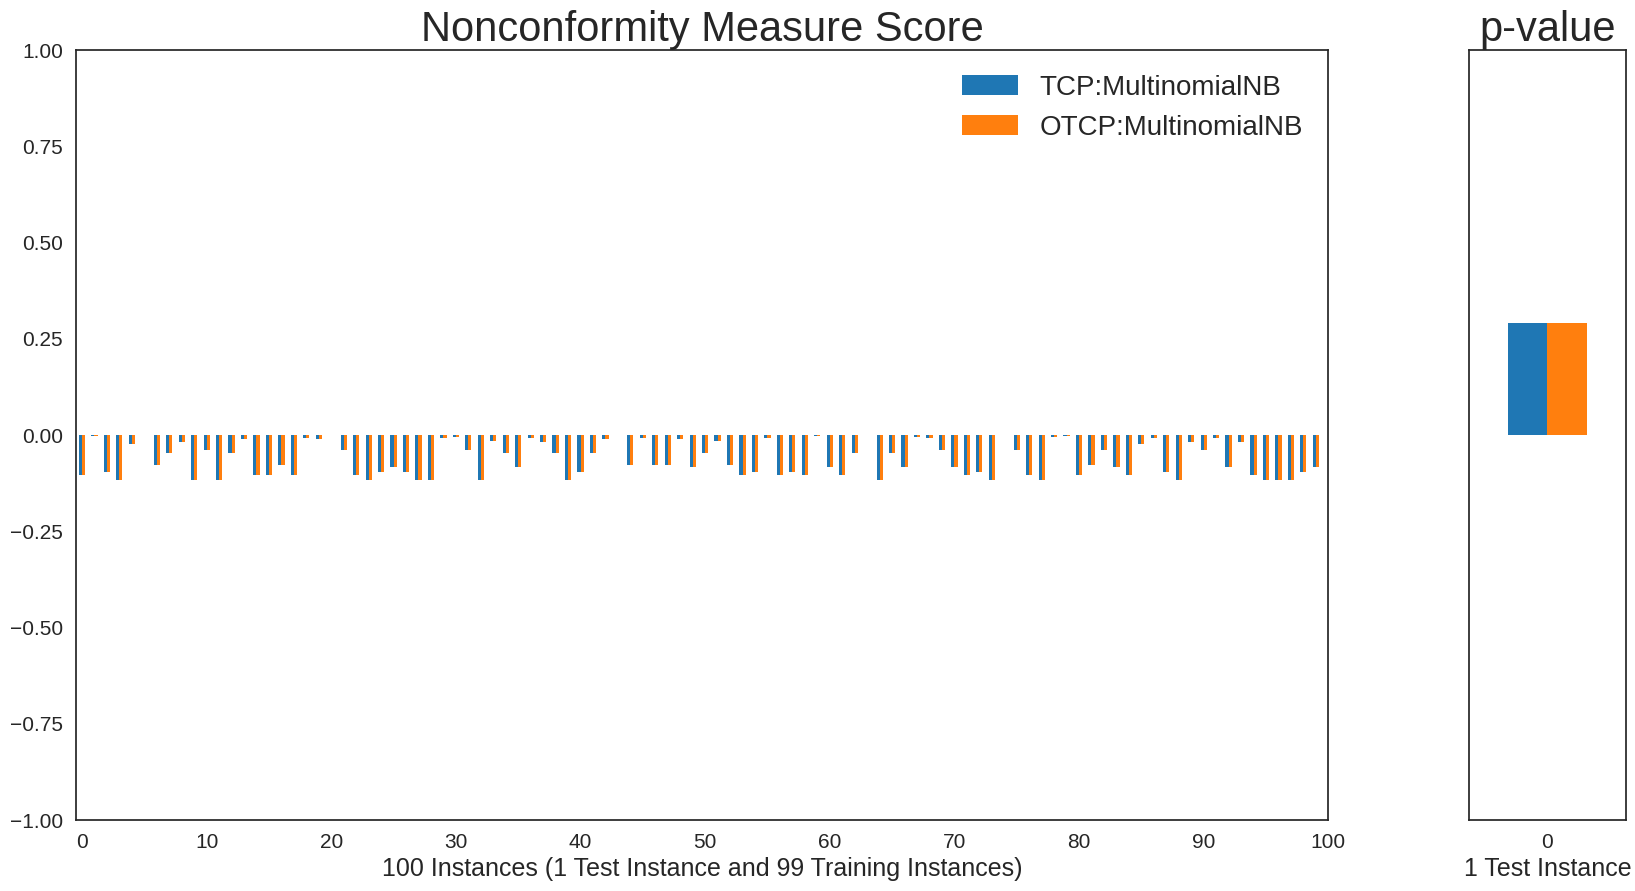
\includegraphics[width = 13cm]{figures/ConsistencyTest_1.png}
    \caption{Consistency Test of TCP and OTCP based on MultinomialNB}
    \label{fig:ConsistencyTest_1}
\end{figure}

\begin{figure}[H]
    \centering
    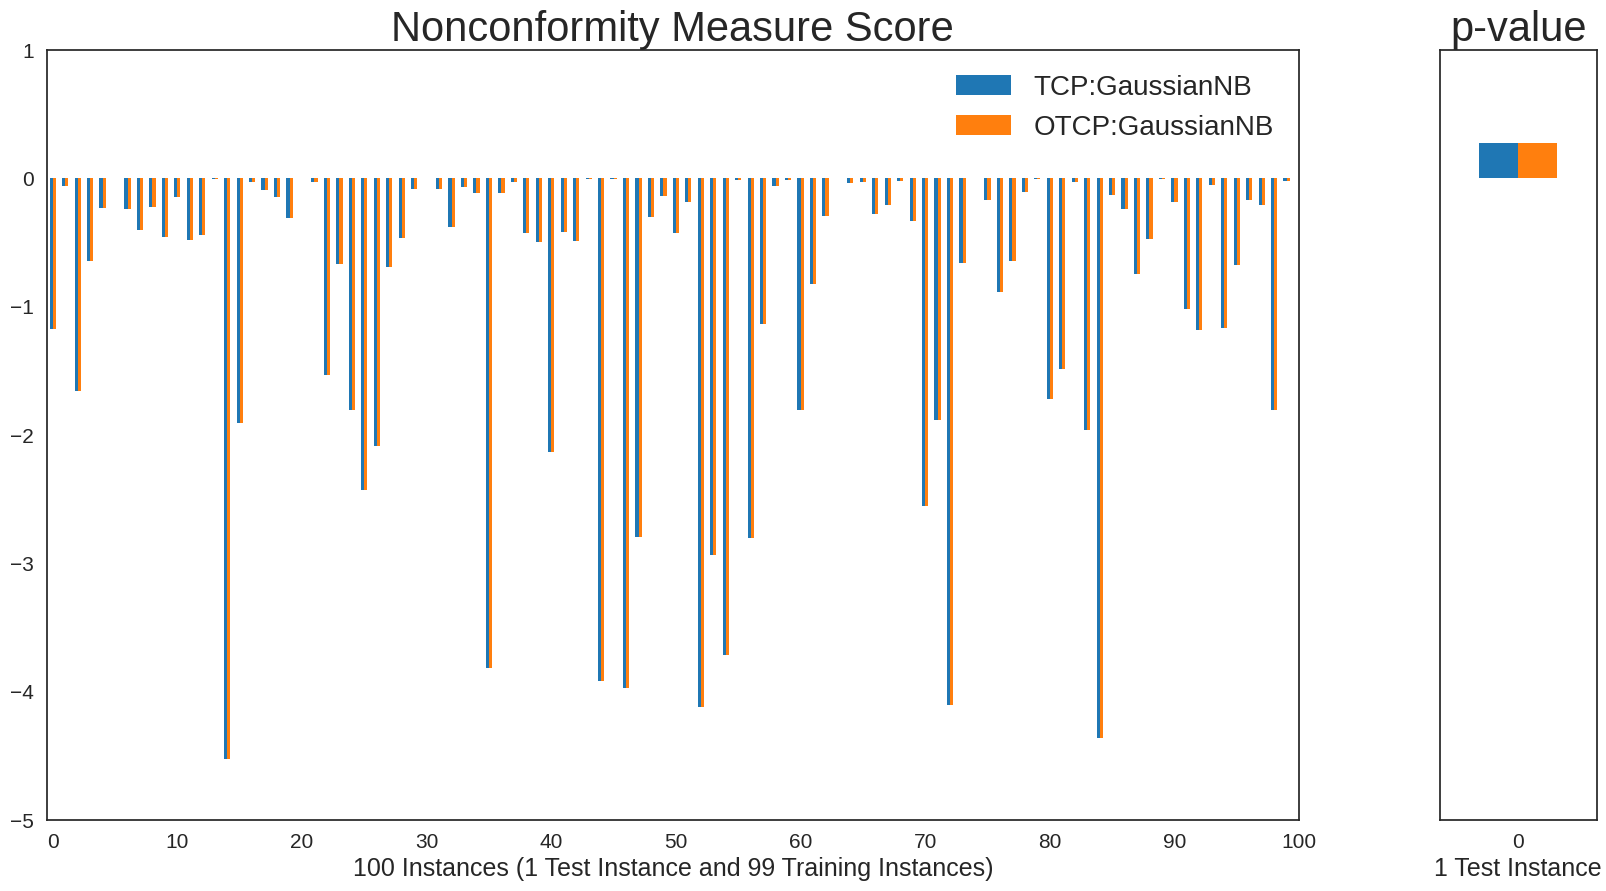
\includegraphics[width = 13cm]{figures/ConsistencyTest_2.png}
    \caption{Consistency Test of TCP and OTCP based on GaussianNB}
    \label{fig:ConsistencyTest_2}
\end{figure}

\subsection{Research Question 2}

Figure \ref{fig:TrainingTime_1} and Figure \ref{fig:AveragePredictionTime_1} show the computational performance between TCP and OTCP based on MultinomialNB or GaussianNB, that is, training time for the classifier and average prediction time for one test instance against the size of the training dataset.\\

\noindent The figures provide insights into the second research question regarding the potential reduction in training and prediction times achieved by OTCP. In terms of training time, standard TCP do not necessitate pre-training a classifier, whereas OTCP require training a classifier in advance. As a result, the training time for standard TCP is considerably shorter than that of their optimized counterparts. Regarding average prediction time, OTCP demonstrate a significant reduction, often by at least one order of magnitude, compared to standard TCP. This improvement in prediction time showcases the efficiency gains achieved through the optimization technique employed.\\

\noindent For the training dataset with 1000 training instances, the training time for OTCP:MultinomialNB amounts to 2.67 seconds, whereas OTCP:GaussianNB requires 12.32 seconds. In contrast, TCP:MultinomialNB and TCP:GaussianNB exhibit training times of less than 0.001 seconds. During the prediction phase, OTCP:MultinomialNB achieves a prediction in approximately 0.97 seconds, while TCP:MultinomialNB requires around 206.12 seconds. Similarly, OTCP:GaussianNB demonstrates a prediction time of 5.24 seconds, compared to the 369.80 seconds of TCP:GaussianNB. 

\begin{figure}[H]
    \centering
    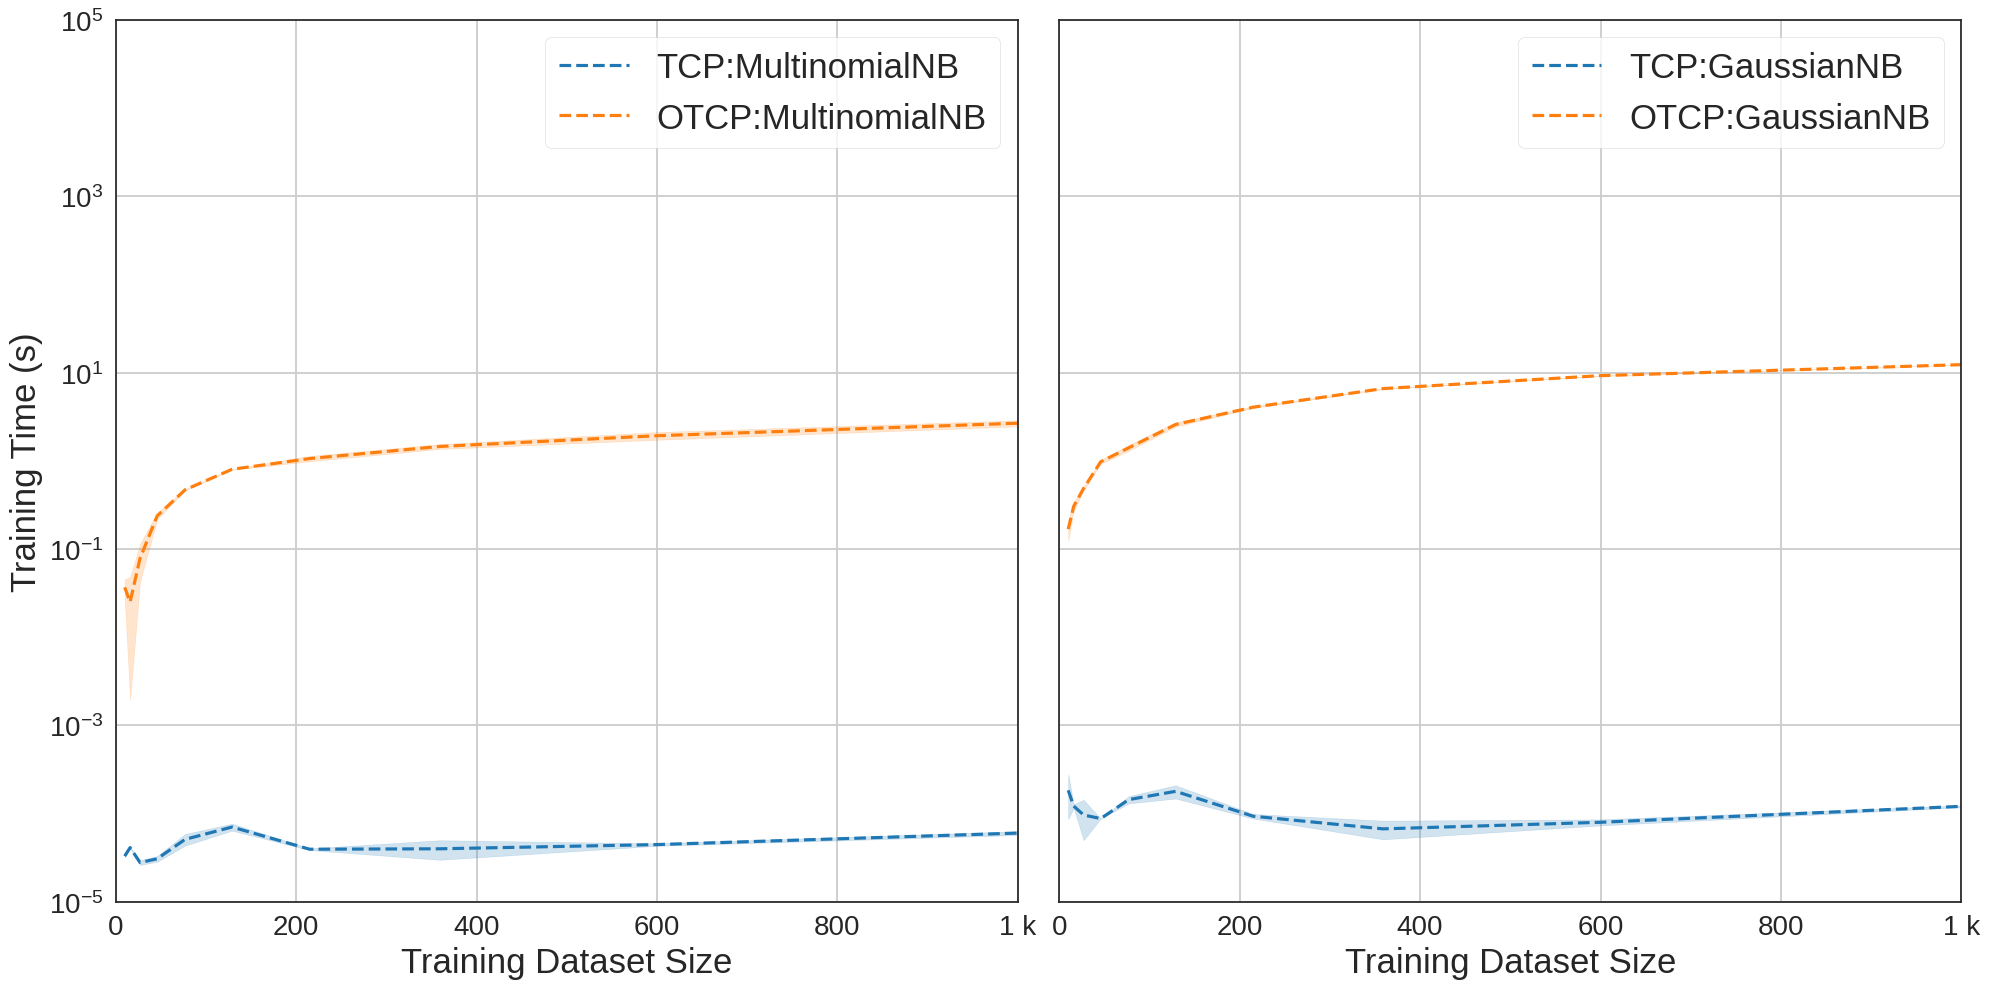
\includegraphics[width = 13cm]{figures/TrainingTime_1.png}
    \caption{Training Time between TCP and OTCP based on MultinomialNB (left) as well as between TCP and OTCP based on GaussianNB (right)}
    \label{fig:TrainingTime_1}
\end{figure}

\begin{figure}[H]
    \centering
    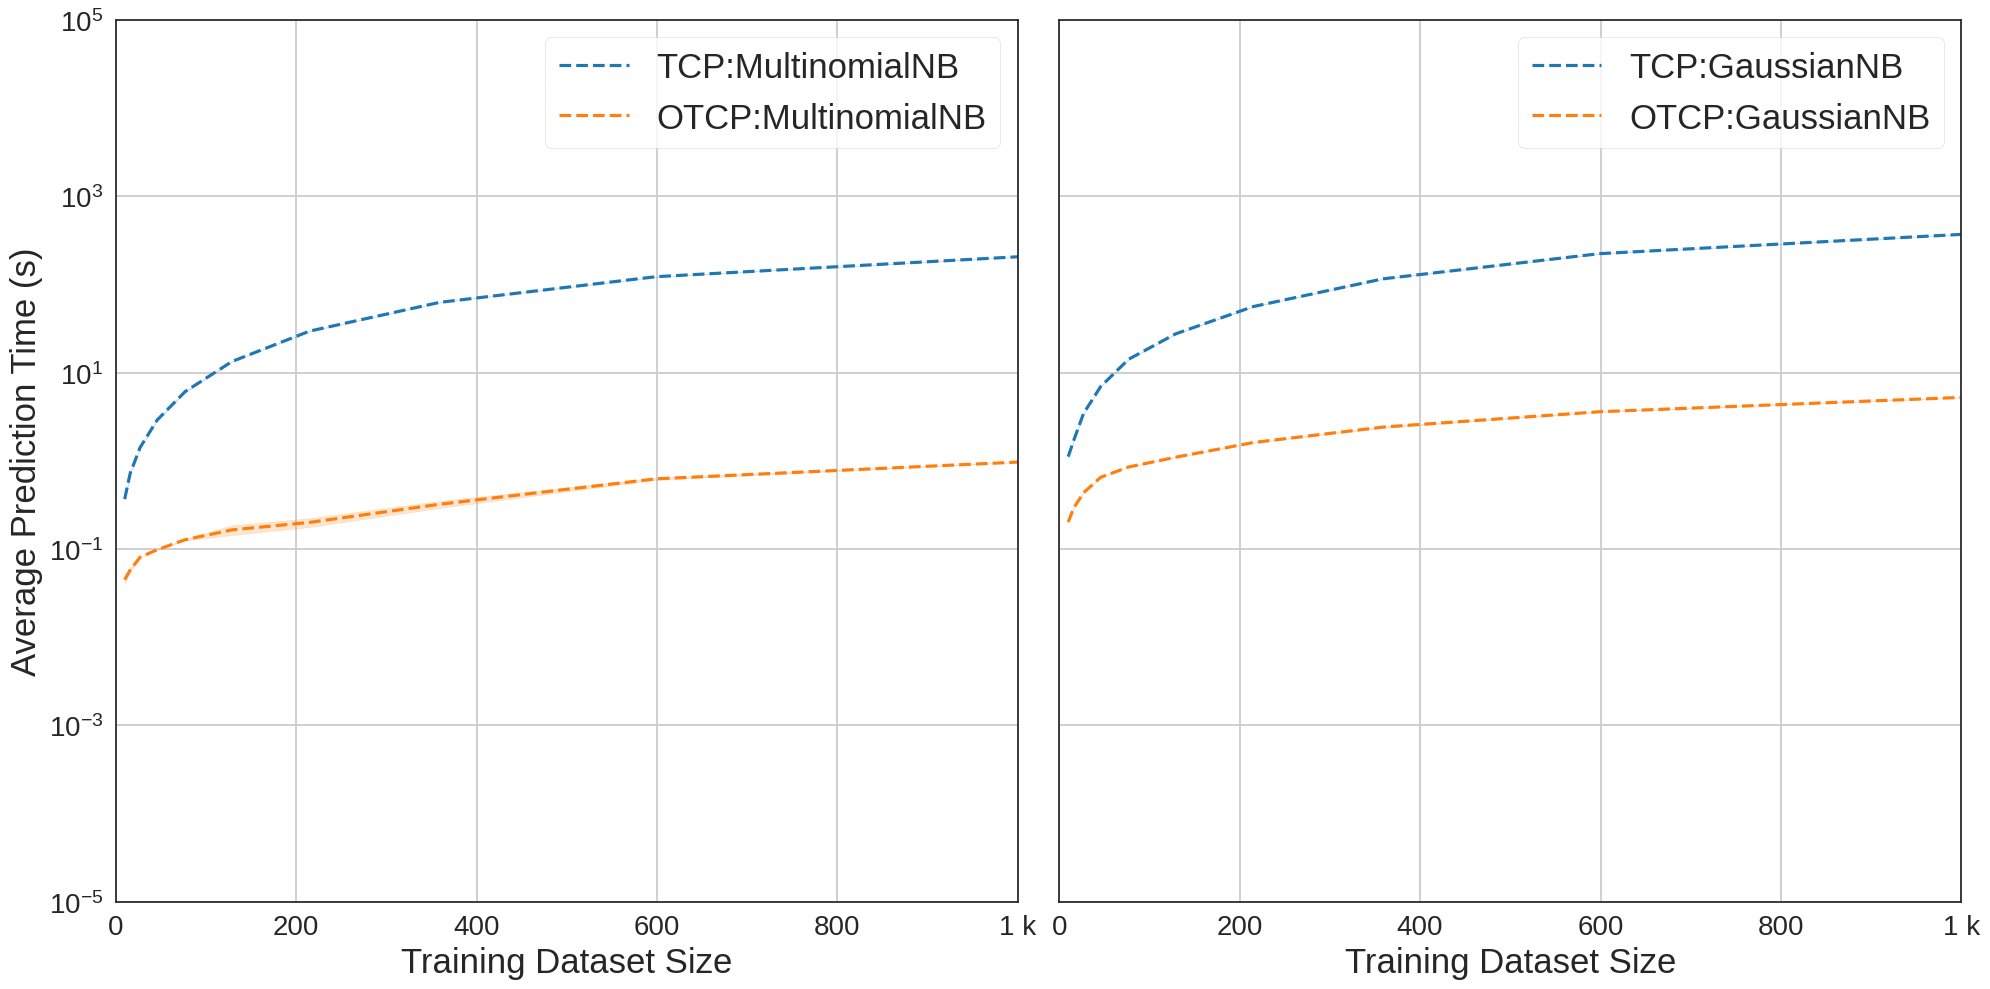
\includegraphics[width = 13cm]{figures/AveragePredictionTime_1.png}
    \caption{Average Prediction Time between TCP and OTCP based on MultinomialNB (left) as well as between TCP and OTCP based on GaussianNB (right)}
    \label{fig:AveragePredictionTime_1}
\end{figure}


\subsection{Research Question 3}

Figure \ref{fig:TrainingTime_2} and Figure \ref{fig:AveragePredictionTime_2} illustrate the computational performance comparison among various OTCP. Specifically, these two figures depict the training time for the classifier and the average prediction time for a single test instance, both plotted against the size of the training dataset. The four OTCP utilize different underlying ML methods, including MultinomialNB, GaussianNB, k-NN, and KDE.\\

\noindent Among the OTCP, k-NN exhibits the highest training time, which aligns with the time complexity analysis results presented in Table \ref{tab:TCA_2}. Following k-NN, GaussianNB demonstrates the second-highest training time. When comparing MultinomialNB and KDE, the training time for KDE increases at a faster rate overall and surpasses MultinomialNB when the training dataset reaches 15,000 instances. Considering the growth trend observed between KDE and GaussianNB, it is expected that KDE's training time will eventually surpass that of MultinomialNB as the training dataset size exceeds 25,000 instances.\\

\noindent Regarding average prediction time, GaussianNB consistently exhibits the highest values, which can be attributed to the complex calculations involved in estimating the likelihood. Conversely, k-NN demonstrates the lowest prediction time among the four OTCP, maintaining this advantage until the training dataset reaches 25,000 instances. In terms of MultinomialNB and KDE, their average prediction times follow a similar increasing trend. Towards the end of the experiments, MultinomialNB slightly surpasses KDE in terms of prediction time, albeit with a marginal difference.

\begin{figure}[H]
    \centering
    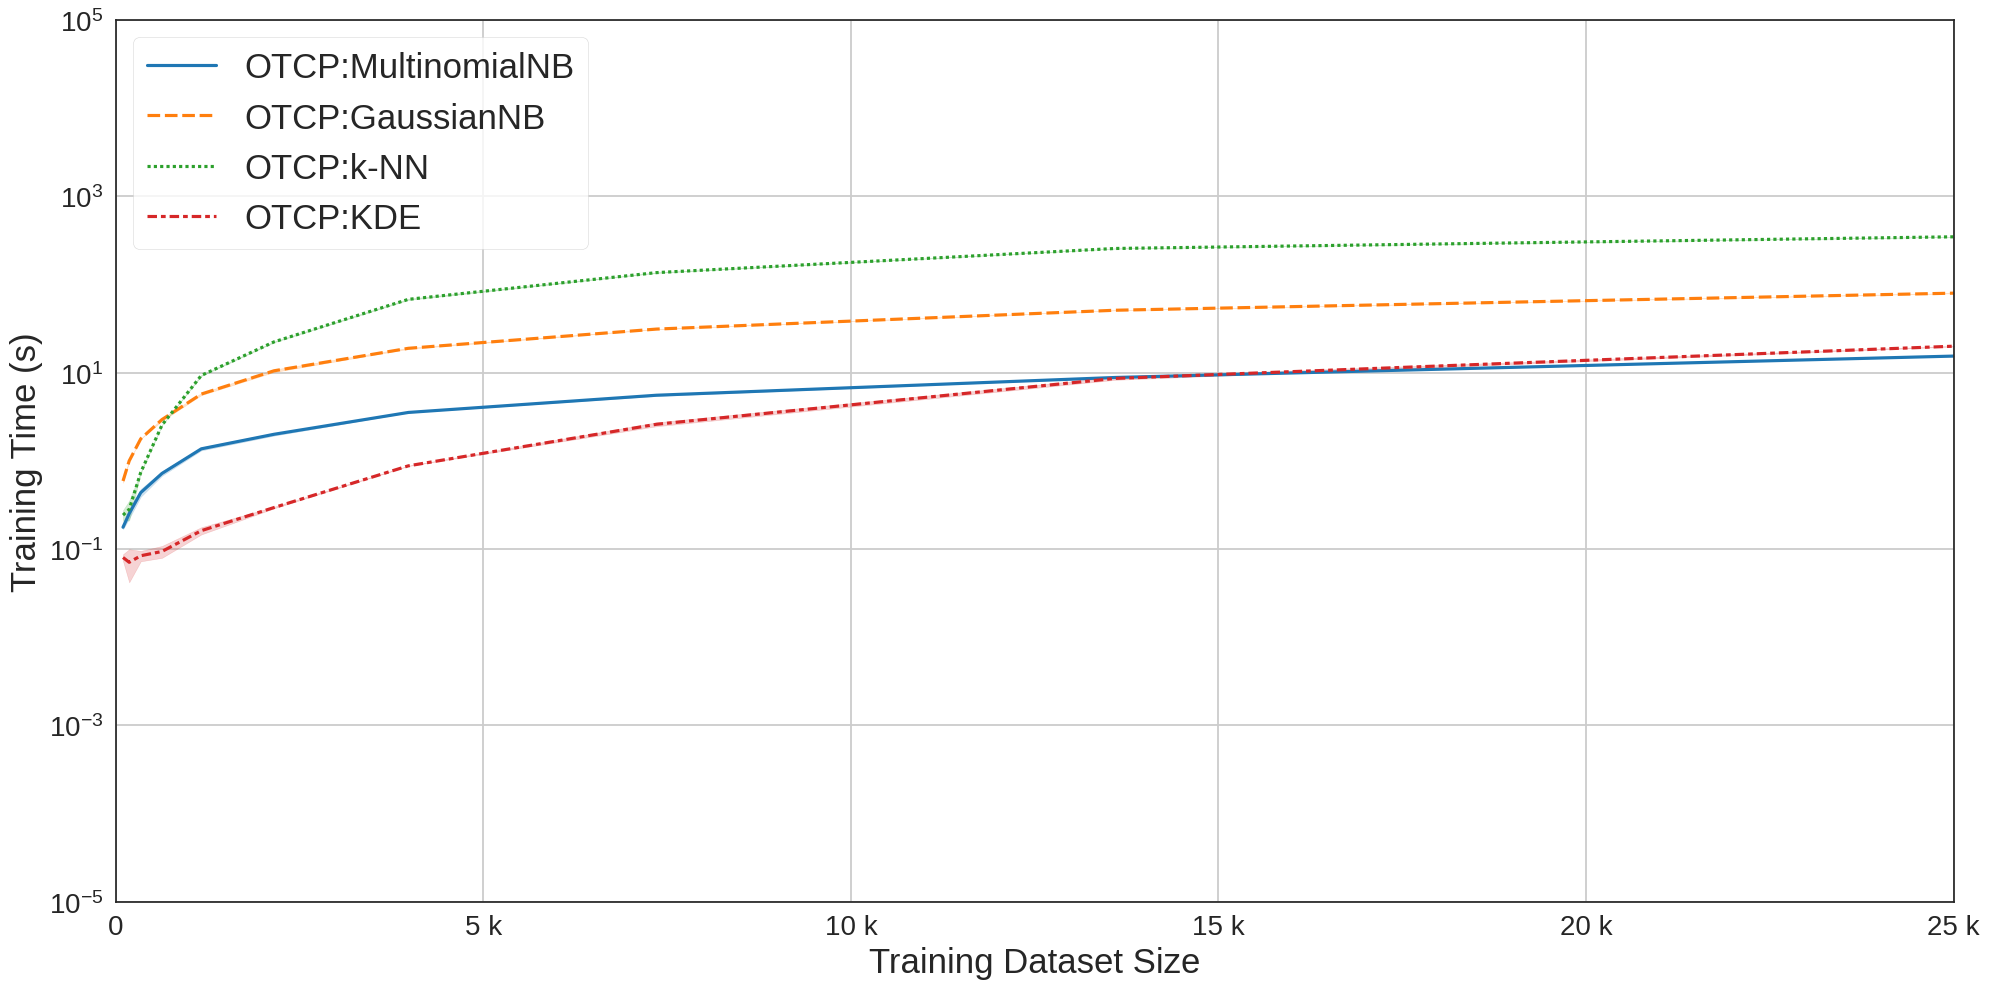
\includegraphics[width = 13cm]{figures/TrainingTime_2.png}
    \caption{Training Time among OTCP based on Different ML Methods}
    \label{fig:TrainingTime_2}
\end{figure}

\begin{figure}[H]
    \centering
    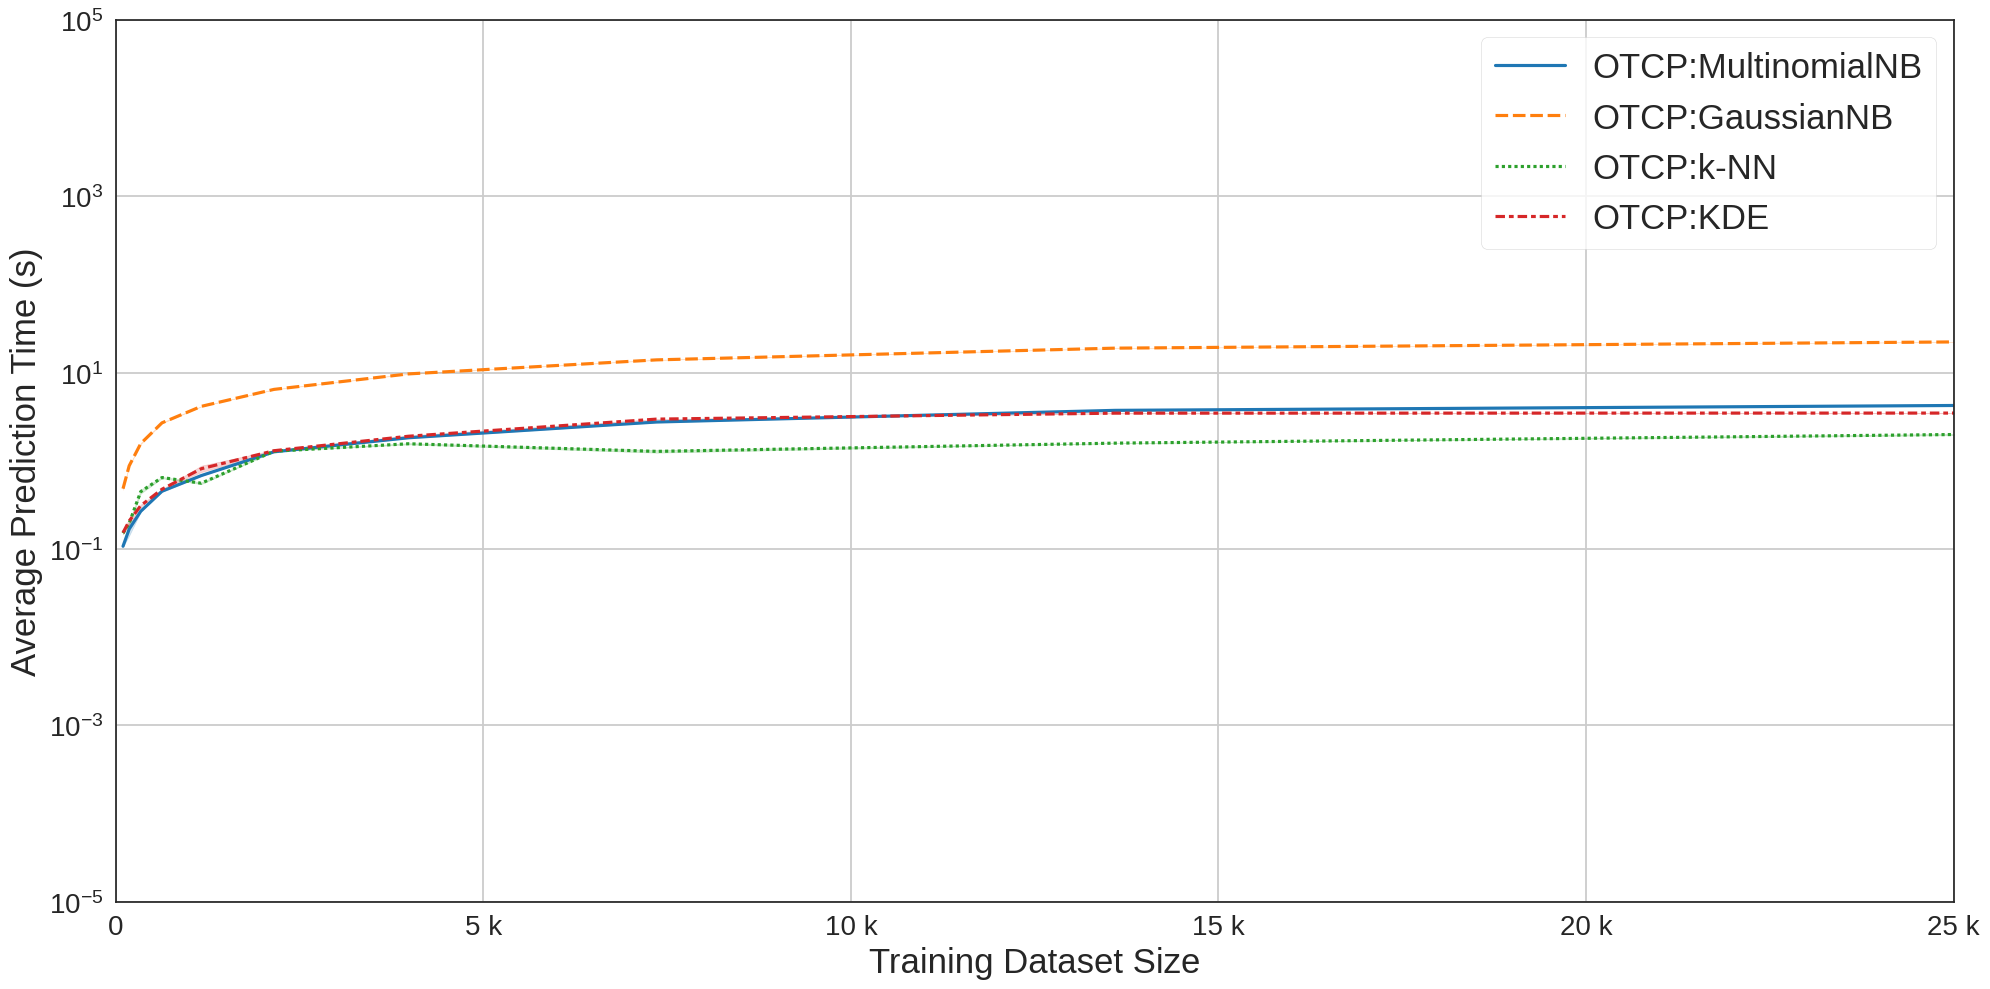
\includegraphics[width = 13cm]{figures/AveragePredictionTime_2.png}
    \caption{Average Prediction Time among OTCP based on Different ML Methods}
    \label{fig:AveragePredictionTime_2}
\end{figure}

\section{Conclusion}

In this chapter, we first verified the correctness of MultinomialNB and GaussianNB. Following this, we proceeded to design an experiment to address the first research question. Through analysis of the experimental results, we concluded that OTCP employing MultinomialNB or GaussianNB produce identical solutions to the standard TCP.\\

\noindent Subsequently, we conducted additional experiments to compare the computational performance across different algorithms, aiming to address the remaining two research questions. Based on the comparison between TCP and OTCP based on MultinomialNB or GaussianNB, we determined that OTCP utilizing NBC exhibit a significant reduction in prediction time compared to the standard TCP. However, there was no point of comparison for training time because standard approaches do not have the training phase. Furthermore, when comparing the performance of various OTCP, we were unable to conclusively determine whether the OTCP based on MultinomialNB or GaussianNB is the fastest algorithm. It is important to note that conducting experiments with larger datasets is necessary to obtain more robust results.

\chapter{Conclusion}
\section{Conclusions}

The computational cost of TCP primarily arises from its key steps (lines 2-4, Algorithm \ref{alg:TCP}), which encompasses the execution of the LOO procedure. In this work, we presented an optimized TCP that utilizes NBC as the nonconformity measure scorer. The main idea revolves around efficiently learning and unlearning an instance, rather than iteratively training a new classifier. Specifically, we optimized TCP based on MultinomialNB for discrete variables and TCP based on GaussianNB for continuous variables.\\

\noindent By thoroughly analyzing the results of the experiments conducted, we have answered the following three research questions.

\begin{itemize}
\item Can the optimized Transductive Conformal Predictors based on Naive Bayes Classifier produce the same exact solutions as standard ones?
\end{itemize}

\noindent The answer to the first question is positive: the consistency test conducted between the standard and optimized TCP demonstrates that both approaches yield identical solutions. 

\begin{itemize}
\item Can the optimized Transductive Conformal Predictors based on Naive Bayes Classifier reduce the training time and prediction time significantly?
\end{itemize}

\noindent Regarding the second research question, it should be noted that a direct comparison of training time between standard and optimized TCP is not theoretically feasible, as the former requires training the classifier for each labelled instance. However, it is noteworthy that both optimized TCP based on MultinomialNB and GaussianNB, consistently exhibit a substantial reduction in prediction time, by at least one order of magnitude compared to standard TCP.

\begin{itemize}
\item Can the optimized Transductive Conformal Predictors based on Naive Bayes Classifier reduce more training time and prediction time than other optimized TCP based on different ML methods?
\end{itemize}

\noindent In regards to the third research question, it is evident from Table \ref{tab:TCA_2} that OTCP based on k-NN has the highest training time complexity, denoted as $O(N^2logN + N^2P)$. This finding aligns with the experimental results depicted in Figure 4.5. Additionally, OTCP based on KDE also incorporates the $N^2$ term in its time complexity, yet its training time does not rank as the second highest. Surprisingly, it even takes slightly longer than MultinomialNB in the case of 25,000 instances. The reason behind this discrepancy may stem from the relatively small size of the experimental training dataset, which prevents a clear distinction between the two approaches. Regarding OTCP based on MultinomialNB and GaussianNB, in theory, GaussianNB ($O(NP+PL)$) should exhibit slightly faster training time than MultinomialNB ($O(NP+PLV)$). However, the experimental results do not align with this theoretical expectation. This inconsistency may arise from the complex calculation involved in estimating the likelihood for GaussianNB.\\

\noindent  In terms of prediction time, it is theoretically expected that OTCP based on k-NN would have the highest time complexity due to the term $NPL$ in $O(NPL+Nl)$. However, contrary to this expectation, the experimental results presented in Figure 4.6 demonstrate that k-NN is the fastest among the tested methods. OTCP based on KDE is characterized by a complexity of $O(NP+NL+L^2)$, while both MultinomialNB and GaussianNB exhibit a complexity of $O(NP+NL+PL)$. This implies that OTCP based on KDE should be faster than MultinomialNB and GaussianNB when the number of classes $L$ is less than the number of input variables $P$, and vice versa. In our experiments, where $L$ is 10 and $P$ is 30, KDE indeed outperforms MultinomialNB and GaussianNB in terms of speed.\\

\noindent The experimental results show slight discrepancies compared to the time complexity analysis results. We attribute these differences to the limitations imposed by the available computational resources, preventing us from conducting experiments with training instances exceeding 25,000. As a result, a comprehensive investigation of this aspect must be left for future research endeavours.

\section{Future Research}
Future research will be concentrated on two primary directions. The first direction involves the design of optimized TCP that utilize NBC and have the ability to handle mixed input variables, as opposed to exclusively discrete or continuous variables. This approach aims to broaden the applicability and flexibility of TCP based on NBC in handling diverse data types. The second research direction aims to address the limitations posed by computational resources. This will involve conducting experiments to compare various optimized TCP, specifically for datasets comprising at least 100,000 training instances, thereby enabling a comprehensive analysis of their performance.

\bibliographystyle{unsrt}
\bibliography{bibliography}
\addcontentsline{toc}{chapter}{Bibliography}
\end{document}